\documentclass[10pt,xcolor={usenames},fleqn,mathserif,serif]{beamer}

%% colors
\definecolor{bittersweet}{rgb}{1.0, 0.44, 0.37}
\definecolor{brilliantlavender}{rgb}{0.96, 0.73, 1.0}
\definecolor{antiquefuchsia}{rgb}{0.57, 0.36, 0.51}
\definecolor{violetw}{rgb}{0.93, 0.51, 0.93}
\definecolor{Veronica}{rgb}{0.63, 0.36, 0.94}
\definecolor{atomictangerine}{rgb}{1.0, 0.6, 0.4}
\definecolor{darkgray}{rgb}{0.66, 0.66, 0.66}
\definecolor{brightcerulean}{rgb}{0.11, 0.67, 0.84}
\definecolor{cadmiumorange}{rgb}{0.93, 0.53, 0.18}
\definecolor{ochre}{rgb}{0.8, 0.47, 0.13}
\definecolor{midnightblue}{rgb}{0.1, 0.1, 0.44}
\definecolor{lemon}{rgb}{1.0, 0.97, 0.0}
\definecolor{grey}{rgb}{0.7, 0.75, 0.71}
\definecolor{amber}{rgb}{1.0, 0.75, 0.0}
\definecolor{almond}{rgb}{0.94, 0.87, 0.8}
\definecolor{bf}{RGB}{88, 86, 88}
\definecolor{bb}{RGB}{177, 177, 177}

%%%%%% Beamer SetUp
\usepackage{beamersetup}
%%%%%%%%%%%%%%%%%%%%%%%%%%%%%%%%%%% importa pacchetti
\usepackage{usepkg}
%%%%%%%%%%%%%%%%%%%%%%%%%%%%%%%%%%% Funzioni generali
\usepackage{functions}
%http://tex.stackexchange.com/questions/246/when-should-i-use-input-vs-include
\newcommand{\setmuskip}[2]{#1=#2\relax} %%problem usinig mu with calc (req by mathtools) loaded
%%SOURCES
\usepackage{sources}
%\usepackage{length}
%%%%%%%%%%%%%%%%%%%%%%%%%%%%%%%%%%% Funzioni per questo file main
\usepackage{mathOp}
\def\status{coazione}%ripeter
\def\keeptrying{coazione}
\usepackage{LocalF}
%%%%%%%%%%%%%%%%%%%%%%%%%%%%%%%%%
\title{Sistema solare (Beamer)}
% A subtitle is optional and this may be deleted
\subtitle{Pianeti maggiori, pianeti nani, asteroidi (NEO,MB,Kuiper,TNO),comete, sistema pianeta-satellite, anelli, evoluzione dinamica.}

%\author{F.~Author\inst{1} \and S.~Another\inst{2}}
% - Give the names in the same order as the appear in the paper.
% - Use the \inst{?} command only if the authors have different
%   affiliation.

%\institute[Universities of Somewhere and Elsewhere] % (optional, but mostly needed)
%{
% \inst{1}
% Department of Computer Science\\
%  University of Somewhere
%  \and
%  \inst{2}%
%  Department of Theoretical Philosophy\\
%  University of Elsewhere}
% - Use the \inst command only if there are several affiliations.
% - Keep it simple, no one is interested in your street address.

\date{Aprile, \today}
% - Either use conference name or its abbreviation.
% - Not really informative to the audience, more for people (including
%   yourself) who are reading the slides online
% Let's get started
\begin{document}

\begin{comment}
\begin{tikzpicture}%plot tabella esopianeti
\pgfplotstableread{circles.dat}\table
\pgfplotstablegetrowsof{\table}
\pgfmathsetmacro{\M}{\pgfplotsretval-1}%rows
\pgfplotstablegetcolsof{\table}
\pgfmathsetmacro{\N}{\pgfplotsretval-1}%cols

\foreach \row in {0,...,\M}{
          \foreach \col in {0,...,\N}{
                 \pgfplotstablegetelem{\row}{[index]\col}\of\table
                 \ifnum\col=0
                       \xdef\x{\pgfplotsretval}
                 \fi
                 \ifnum\col=1
                       \xdef\y{\pgfplotsretval}
                 \fi
                 \ifnum\col=2
                       \xdef\radius{\pgfplotsretval}
                 \fi
                 }
                 \definecolor{mycolor}{RGB}{\pdfuniformdeviate 256,%
                                            \pdfuniformdeviate 256,%
                                            \pdfuniformdeviate 256}
                 \fill[mycolor,opacity=.5] (\x,\y)circle(\radius cm);
}
\end{tikzpicture}
\end{comment}

\begin{filecontents}{conservedvector.tex}
\centering
\begin{figure}
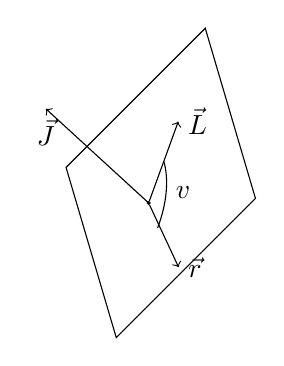
\begin{tikzpicture}[rotate around z=45, rotate around x=-45]
\draw (0,-0.3,0) -- (2.5,-0.3,0) -- (2.5,2.5,0) -- (0,2.5,0) -- cycle;
\draw[->] (1.,1.,0)node[draw,circle,inner sep=0] (o) {} -- (1.5,1.5,2)node[below] {$\vec{J}$};
\draw[->] (o) -- ++(295:0.9cm)node[right] {$\vec{r}$};
\draw[->] (o) -- ++(70:1.1cm)node[right] {$\vec{L}$}node [midway] (aux){};
\draw (aux) arc (0:-50:1) node[midway,right] {$v$};
\end{tikzpicture}
\label{fig:Lenztikz}
\end{figure}
\end{filecontents}

\begin{filecontents}{reducedproblem.tex}
%reduced problem
\begin{tikzpicture}
\node[circle,fill,inner sep=1pt,label=above:M] (M) at (0,0) {}; 
\draw (M)--++(30:1cm) node[circle,fill,inner sep=1pt,label=below:O] (O) {};
\draw[->] (O)--++(30:1.5cm) node[circle,fill,inner sep=1pt,label=above:m,yshift=1pt,xshift=1pt] (m) {} node[midway,above] {$\vec{r}$} ;
\node[circle,fill,inner sep=1pt,below=1cm of O,label=below:O] (O1) {}; 
\draw[->] (O1)--++(30:1.5cm) node[circle,fill,inner sep=1pt,label=above:m,yshift=1pt,xshift=1pt] (m1) {} node[midway,below] {$\vec{r_1}$} ;
\draw[->] (O1)--++(-150:1cm) node[circle,fill,inner sep=1pt,label=above:m,yshift=1pt,xshift=1pt] (m1) {} node[midway,below] {$\vec{r_2}$} ;
%\node (dida) at (7,0) {\parbox{8cm}{Siano m e M due masse puntiformi o a simmetria sferica: O \'e il centro di massa e $\vec{r}=\vec{r_1}-\vec{r_2}$ la distanza relativa.}};
\end{tikzpicture}
\end{filecontents}

\begin{filecontents}{ellipse.tex}
%ellisse
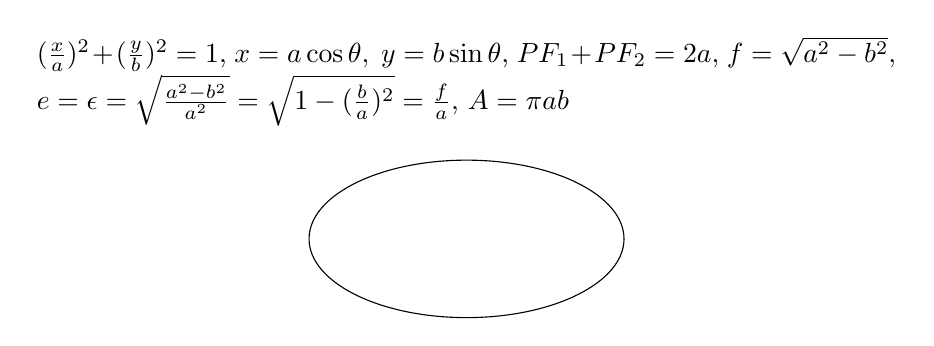
\begin{tikzpicture}
\draw ellipse (2cm and 1cm) node (o) {};
\node (prop) at (0,2) {\parbox{0.9\textwidth}{
$(\frac{x}{a})^2+(\frac{y}{b})^2=1$,
$x=a\cos{\theta},\ y=b\sin{\theta}$,
$PF_1+PF_2=2a$,
$f=\sqrt{a^2-b^2}$,
$e=\epsilon=\sqrt{\frac{a^2-b^2}{a^2}}=\sqrt{1-(\frac{b}{a})^2}=\frac{f}{a}$,
$A=\pi ab$}
};
\end{tikzpicture}
\end{filecontents}%%contain tikz files as filecontents

\addtobeamertemplate{block begin}{\setlength\abovedisplayskip{2pt}\setlength\belowdisplayskip{2pt}\setlength\abovedisplayshortskip{2pt}\setlength\belowdisplayshortskip{2pt}}

\addtobeamertemplate{block begin}{\vspace*{-3pt}}{}
\addtobeamertemplate{block end}{}{\vspace*{-3pt}}

\begin{frame}
  \titlepage
\end{frame}

% Section and subsections will appear in the presentation overview
% and table of contents.
%\frame{\tableofcontents[onlyparts]}

\begin{frame}[]{Sistemi planetari: Sistema solare}\linkdest{argomenti}
\tableofcontents[onlyparts]
\end{frame}

\begin{wordonframe}{Perch\'e studio queste cose?? Sviluppi; futuro.}
Determinazione struttura planetaria.
Test modelli formazione evoluzione, dinamici per  riprodurre caratteristiche sistema solare. sistemi extra-solari.
Sistema Giove e sistema Saturno: modello formazione evoluzione planetario, perturbazioni
\end{wordonframe}

\begin{frame}{Cose da scrivere}
%%\listofframes
\end{frame}


\part{Modello planetario}\linkdest{planetarymodel}
\section{Modello di pianeta}

\subsection{Classificazione.}

\begin{frame}{Sistema solare: pianeti.}
\begin{table}[!ht]
\pgfplotstabletypeset[every head row/.style={
 %before row={},
 %every last row/.style={after row=\bottomrule},
 after row={\midrule}
},
every 2 row/.style={after row=\midrule},
every last row/.style={after row=\bottomrule},
every first column/.style={column type/.add={|}{}},
every last column/.style={column type/.add={}{|}},
%columns/0/.style = {column type/.add={|}{}},
%columns/5/.style = {column type/.add={|}{}},
%columns/0/.style={string type},
display columns/1/.style={column name={mass},string type},
display columns/2/.style={column name={$\bar{\rho}$},clear infinite},
display columns/3/.style={column name={R},clear infinite},
display columns/4/.style={column name={$g_s$},clear infinite},
display columns/5/.style={column name={$J_2$},string type},
display columns/planets/.style={column name={pianeta},string type},
create on use/planets/.style={create col/set list={Mercury, Venus, Earth, Mars, Jupiter, Saturn, Uranus, Neptune}},
columns/planets/.style={string type},
columns={planets, mass, Rp, rhomean, gs, j2},
/pgf/number format/precision=3
     ]{solarsystemmain-pc.txt} %%%
%\captionof{table}{}\label{tab:}
\end{table}
\end{frame}

\begin{frame}{Sistema solare: pianeti nani}
\pgfplotstableread{asteroids.txt}\asteroids
\pgfplotstableread{dwarfplanets.txt}\dwarfplanets
\begin{block}{Asteroidi}
\begin{table}[!ht]
\pgfplotstabletypeset[skip rows between index={1}{27},
every head row/.style={
 %before row={},
 %every last row/.style={after row=\bottomrule},
 after row={\midrule}
},
every 2 row/.style={after row=\midrule},
every last row/.style={after row=\bottomrule},
every first column/.style={column type/.add={|}{}},
every last column/.style={column type/.add={}{|}},
%columns/0/.style = {column type/.add={|}{}},
%columns/5/.style = {column type/.add={|}{}},
%columns/0/.style={string type},
display columns/0/.style={column name={Asteroid},string type},
display columns/1/.style={column name={R (Km)},string type},
display columns/2/.style={column name={mass \SI{e15}{\kilo\gram}},string type},
display columns/3/.style={column name={$P_{rot} (hrs)$},clear infinite},
display columns/4/.style={column name={P (yrs)},clear infinite},
display columns/5/.style={column name={a},clear infinite},
display columns/6/.style={column name={e},clear infinite},
display columns/7/.style={column name={i (deg)},clear infinite},
columns={name, R, mass, spin, P, a, e, i},
/pgf/number format/precision=3
     ]{\asteroids} %%%
%\captionof{table}{Caratteristiche pianeti terrestri.}\label{tab:terrestrial planets}
\end{table}
\end{block}
\begin{block}{plutini}
\begin{table}[!ht]
\pgfplotstabletypeset[every head row/.style={
 %before row={},
 %every last row/.style={after row=\bottomrule},
 after row={\midrule}
},
every 2 row/.style={after row=\midrule},
every last row/.style={after row=\bottomrule},
every first column/.style={column type/.add={|}{}},
every last column/.style={column type/.add={}{|}},
%columns/0/.style = {column type/.add={|}{}},
%columns/5/.style = {column type/.add={|}{}},
%columns/0/.style={string type},
display columns/0/.style={column name={name},string type},
display columns/1/.style={column name={R (Km)},clear infinite},
display columns/2/.style={column name={mass(Earth)},string type},
display columns/3/.style={column name={a},clear infinite},
display columns/4/.style={column name={e},clear infinite},
display columns/5/.style={column name={i (deg)},clear infinite},
columns={name, D, mass, a, e, i},
/pgf/number format/precision=3
     ]{\dwarfplanets} %%%
%\captionof{table}{}\label{tab:}
\end{table}
\end{block}

\end{frame}

\begin{wordonframe}{classificazione: pianeti sistema solare}
Un pianeta ha le seguenti caratteristiche
\begin{itemize}
    \item \'E in orbita attorno ad una stella di riferimento.
    \item \'E abbastanza massiccio da essere dominato dalle forze di gravit\'a: forma di equilibrio ''idrostatica''.
    \item Ha completamente ripulito la regione del sistema intorno alla sua orbita. Altrimenti \'e un pianeta nano.
\end{itemize}

\end{wordonframe}


\subsection{Energia assorbita. Temperatura efficace/Radiative transfer}

Suppongo una distribuzione uniforme sulla superficie del pianeta.

La temperatura efficace del pianeta nell'approssimazione di corpo nero
\begin{align*}
&4\pi R_P^2\sigma T_{eff,P}^4=(1-A)\frac{L^*R_P^2}{4r_{P*}^2}\\
&=(1-A)\frac{\pi R_*^2T_{eff,*}^4}{r_{P*}^2}R_P^2\\
&T_{eff,P}=(\frac{1-A}{A})\expy{\frac{1}{4}}(\frac{R_*}{r_{P*}})\expy{\frac{1}{2}}T_{eff,*}
\end{align*}

Approssimazioni successive
\begin{itemize}
    \item Correzione all'approssimazione di corpo nero: corpo grigio. Tengo conto degli effetti di riflessione (corpo nero: assorbimento perfetto).
    \item Differenza di temperatura tra regioni illuminate e non del pianeta: modello termico. Regioni polari meno illuminate cio\'e pi\'u fredde: \'e vero se l'asse di rotazione \'e ortogonale al piano dell'orbita (non vale per Urano).
    
    Per corpi con rotazione veloce o con atmosfera l'escursione termica \'e modesta.
    
    Equilibrio termico locale. Nel punto della superficie in cui il Sole \'e allo zenit: $T_{s*}=(\frac{R_*}{r_{P*}})\expy{\frac{1}{2}}T_{eff,*}$.
\end{itemize}
                


\part{Fenomenologia sistema solare: caratteristiche principali. Pianeti terrestri, giganti gassosi, giganti ghiacciati, sistemi di anelli satelliti e corpi minori}\linkdest{solsys}

\begin{frame}{this part toc}
\begin{itemize}
\item Pianeti terrestri
\item Giganti gassosi: Giove e Saturno
\item Giganti ghiacciati: Urano, Nettuno
\item Asteroidi: NEO, MB, TNO. Comete. Anelli
\end{itemize}
\end{frame}

\section{Terrestrial planets}\linkdest{terrestrials}
\subsection{Overview terrestrial planets}

%solarsystemmain-orbit: dps e i P% spin
%solarsystemmain-pc: mass 	  rhomean Rp   gs  j2
%solarsystemmain-th: A 	 Teff TeffA Tss  H	  atms
%display columns/1/.style={column name={$r_{p\odot}(\SI{e8}{\kilo\meter})$},clear infinite},
%display columns/2/.style={column name={$R_p\SI{e3}{\kilo\meter}$},clear infinite},
%display columns/3/.style={column name={albedo},clear infinite},
%display columns/4/.style={column name={$T_{eff,p}$},clear infinite},
%display columns/5/.style={column name={$T_{eff,p}'$},clear infinite},
%display columns/6/.style={column name={$T_{ss}$},clear infinite},
%display columns/7/.style={column name={$m_V^{opp}$},clear infinite},
%display columns/8/.style={column name={H},clear infinite},


\begin{frame}{Caratteristiche principali}
\begin{table}[!ht]
\pgfplotstabletypeset[skip rows between index={4}{8},
every head row/.style={
 %before row={},
 %every last row/.style={after row=\bottomrule},
 after row={\midrule}
},
every 2 row/.style={after row=\midrule},
every last row/.style={after row=\bottomrule},
every first column/.style={column type/.add={|}{}},
every last column/.style={column type/.add={}{|}},
%columns/0/.style = {column type/.add={|}{}},
%columns/5/.style = {column type/.add={|}{}},
%columns/0/.style={string type},
display columns/1/.style={column name={$r_{p\odot}(\SI{e8}{\kilo\meter})$},clear infinite},
display columns/2/.style={column name={e},clear infinite},
display columns/3/.style={column name={i},clear infinite},
display columns/4/.style={column name={$\tau_{sid}$},clear infinite},
display columns/5/.style={column name={obliquity},clear infinite},
display columns/planets/.style={column name={pianeta},string type},
create on use/planets/.style={create col/set list={Mercury, Venus, Earth, Mars}},
columns/planets/.style={string type},
columns={planets, dps, e, i, Ps, obl},
/pgf/number format/precision=3
     ]{solarsystemmain-orbit.txt} %%%
%\captionof{table}{Caratteristiche pianeti terrestri.}\label{tab:terrestrial planets}
\begin{itemize}
\item Accretion of planetesimal
\item Ratation depends upon fine details (i, e,\ldots)
\end{itemize}
\end{table}
\end{frame}

\begin{wordonframe}{Pianeti terrestri: overview}
\begin{itemize}\item Hill interior/exterior orbits are symmetric: positive/negative angular momentum is equally likely
\item Formation from planetesimal accretion; slow accretion deprived the regions from material to form satellites.

\end{itemize}
\end{wordonframe}

\subsection{Mercury}

%\begin{frame}{Mercurio:}
%\end{frame}
%\begin{wordonframe}{struttura}
%\end{wordonframe}

\subsection{Venus}

%\begin{frame}{Venus: Spin/runaway greenhouse}
%\end{frame}
%\begin{wordonframe}{struttura}
%\end{wordonframe}

\subsection{Sistema Terra-Luna}
\tolbf
\begin{frame}{Sistema Terra/Luna
Formation scenarios:
\end{frame}

\begin{wordonframe}{Terra/Luna}

\end{wordonframe}

\subsection{Marte}

%\begin{frame}{Mars: satellites}
%Phobos, Deimos: tidal evolution inward outward
%\end{frame}
%\begin{wordonframe}{struttura}
%\end{wordonframe} 

\section{Giant planets}\linkdest{giants}
\subsection{Caratteristiche pianeti giganti}

\begin{frame}{Pianeti giganti: caratteristiche orbitali}\tolbf
\begin{table}[!ht]
\pgfplotstabletypeset[skip rows between index={0}{4},
every head row/.style={
 %before row={},
 %every last row/.style={after row=\bottomrule},
 after row={\midrule}
},
every 2 row/.style={after row=\midrule},
every last row/.style={after row=\bottomrule},
every first column/.style={column type/.add={|}{}},
every last column/.style={column type/.add={}{|}},
%columns/0/.style = {column type/.add={|}{}},
%columns/5/.style = {column type/.add={|}{}},
%columns/0/.style={string type},
display columns/1/.style={column name={$r_{p\odot}(\SI{e8}{\kilo\meter})$},clear infinite},
display columns/2/.style={column name={e},clear infinite},
display columns/3/.style={column name={i},clear infinite},
display columns/4/.style={column name={$\tau_{sid}$},clear infinite},
display columns/5/.style={column name={obliquity},clear infinite},
display columns/planets/.style={column name={pianeta},string type},
create on use/planets/.style={create col/set list={Mercury, Venus, Earth, Mars,Jupiter,Saturn,Uranus, Neptune}},
columns/planets/.style={string type},
columns={planets, dps, e, i, Ps, obl},
/pgf/number format/precision=3
     ]{solarsystemmain-orbit.txt} %%%
%\captionof{table}{Caratteristiche pianeti giganti.}\label{tab:terrestrial planets}
\end{table}
\end{frame}

\subsection{Jupiter system.}

\begin{frame}{Resonances (da distribuire)}


The resonance ensures that, when they approach perihelion and Neptune's orbit, Neptune is consistently distant (averaging a quarter of its orbit away). Other (much more numerous) Neptune-crossing bodies that were not in resonance were ejected from that region by strong perturbations due to Neptune. There are also smaller but significant groups of resonant trans-Neptunian objects occupying the 1:1 (Neptune trojans), 3:5, 4:7, 1:2 (twotinos) and 2:5 resonances, among others, with respect to Neptune.

The Titan Ringlet within Saturn's C Ring represents another type of resonance in which the rate of apsidal precession of one orbit exactly matches the speed of revolution of another. The outer end of this eccentric ringlet always points towards Saturn's major moon Titan.

A Kozai resonance occurs when the inclination and eccentricity of a perturbed orbit oscillate synchronously (increasing eccentricity while decreasing inclination and vice versa). This resonance applies only to bodies on highly inclined orbits; as a consequence, such orbits tend to be unstable, since the growing eccentricity would result in small pericenters, typically leading to a collision or (for large moons) destruction by tidal forces.

A Laplace resonance is a three-body resonance with a 1:2:4 orbital period ratio (equivalent to a $4:2:1$ ratio of orbits). The term arose because Pierre-Simon Laplace discovered that such a resonance governed the motions of Jupiter's moons Io, Europa, and Ganymede. It is now also often applied to other 3-body resonances with the same ratios, such as that between the extrasolar planets Gliese 876 c, b, and e. Three-body resonances involving other simple integer ratios have been termed "Laplace-like" or "Laplace-type".

A Lindblad resonance drives spiral density waves both in galaxies (where stars are subject to forcing by the spiral arms themselves) and in Saturn's rings (where ring particles are subject to forcing by Saturn's moons).

Several prominent examples of secular resonance involve Saturn. A resonance between the precession of Saturn's rotational axis and that of Neptune's orbital axis (both of which have periods of about 1.87 million years) has been identified as the likely source of Saturn's large axial tilt ($26.7\deg$). Initially, Saturn probably had a tilt closer to that of Jupiter ($3.1\deg$). The gradual depletion of the Kuiper belt would have decreased the precession rate of Neptune's orbit; eventually, the frequencies matched, and Saturn's axial precession was captured into the spin-orbit resonance, leading to an increase in Saturn's obliquity. (The angular momentum of Neptune's orbit is 104 times that of Saturn's spin, and thus dominates the interaction.)

Examples are the $1:2:4$ resonance of Jupiter's moons Ganymede, Europa and Io, and the $2:3$ resonance between Pluto and Neptune. Unstable resonances with Saturn's inner moons give rise to gaps in the rings of Saturn. The special case of 1:1 resonance (between bodies with similar orbital radii) causes large Solar System bodies to eject most other bodies sharing their orbits; this is part of the much more extensive process of clearing the neighbourhood, an effect that is used in the current definition of a planet.

The Titan Ringlet within Saturn's C Ring represents another type of resonance in which the rate of apsidal precession of one orbit exactly matches the speed of revolution of another. The outer end of this eccentric ringlet always points towards Saturn's major moon Titan.

A Kozai resonance occurs when the inclination and eccentricity of a perturbed orbit oscillate synchronously (increasing eccentricity while decreasing inclination and vice versa). This resonance applies only to bodies on highly inclined orbits; as a consequence, such orbits tend to be unstable, since the growing eccentricity would result in small pericenters, typically leading to a collision or (for large moons) destruction by tidal forces.

In an example of another type of resonance involving orbital eccentricity, the eccentricities of Ganymede and Callisto vary with a common period of 181 years, although with opposite phases.

\end{frame}


\begin{frame}{Giove}


\end{frame}

\begin{wordonframe}{giove}
Il diametro di Giove $D_G\approx\SI{e5}{\kilo\meter}$ visto dalla terra sottende angolo $\alpha\approx\SI{1.5e-4}{\radian}=\ang{;;30}$.

Caratteristiche dell'orbita:
\begin{itemize}
    \item $\Pi_{360}\approx\SI{12}{\year}$.
    \item $d_{G\odot}\approx\SI{5}{\astronomicalunit}$.
    \item $e=0.048$ ($d(P,F)=ed(P,r), b^2=(1-e^2)a^2$)
\end{itemize}
\end{wordonframe}



\subsection{Saturn system.}

\subsection{Uranus}


\subsection{Neptune}



\section{Corpi minori: Asteroidi, TNO, comete. Anelli planetarii}\linkdest{asteroidscomets}
\subsection{Corpi minori del sistema solare}

\begin{frame}{Corpi minori: origine ed evoluzione.}
\begin{itemize}
\item MB: \num{e5} asteroids, $M_{T}\approx\num{5e-4}\mearth{}$: less mass than expected from smooth distribution in primordial nebula.
\item Why there is so little mass remaining in asteroid region ($\approx\SI{3}{\astronomicalunit}$)? 
\item Why is this mass spread over so many body??
\item Why most of asteroid orbits are more inclinated/eccentric than that of major planets?
\item Why are asteroid so compositionally diverse?
\item Satelliti e anelli
\item Kuiper Belt require that planetesimal exist beyond Neptune; Why the abrupt cut-oof beyond Neptune?
\item Oort cloud: Mass of solid material eject from planetary (giants) region \numrange{1}{1000}$\mearth{}$
\end{itemize}
\end{frame}

\begin{wordonframe}{Asteroidi, comete, TNO, ogetti della fascia di Kuiper-Edgeworth.}
In asteroid regions there is 2-3 order of magnitude less mass than expected from smooth mass distribution in primordial nebula.

Orbital resonances can also destabilize one of the orbits. For small bodies, destabilization is actually far more likely.

Secular resonances: mean drift of pericentre becomes commensurable with one of proper frequency of planetary system

In the asteroid belt beyond 3.5 AU from the Sun, the 3:2, 4:3 and 1:1 resonances with Jupiter are populated by clumps of asteroids (the Hilda family, the few Thule asteroids, and the extremely numerous Trojan asteroids, respectively).
\end{wordonframe}

\subsection{Asteroidi. Main Belt.}\linkdest{asteroids}

\begin{frame}{Caratteristiche main belt}
\begin{columns}[T]\begin{column}{0.5\textwidth}
\begin{block}{Classificazione fotometrica}
\begin{itemize}
    \item C: Condriti carbonacee. Low albedo, flat spectrum in V-NIR.
    \item S: high albedo, silicates absorption band
    \item D-type: very red (low temperature, organic compounds: $CH_4$, etc)
    \item M-type: $A\approx0.1$, reddish
\end{itemize}
\end{block}
\end{column}\begin{column}{0.5\textwidth}
\begin{figure}[!ht]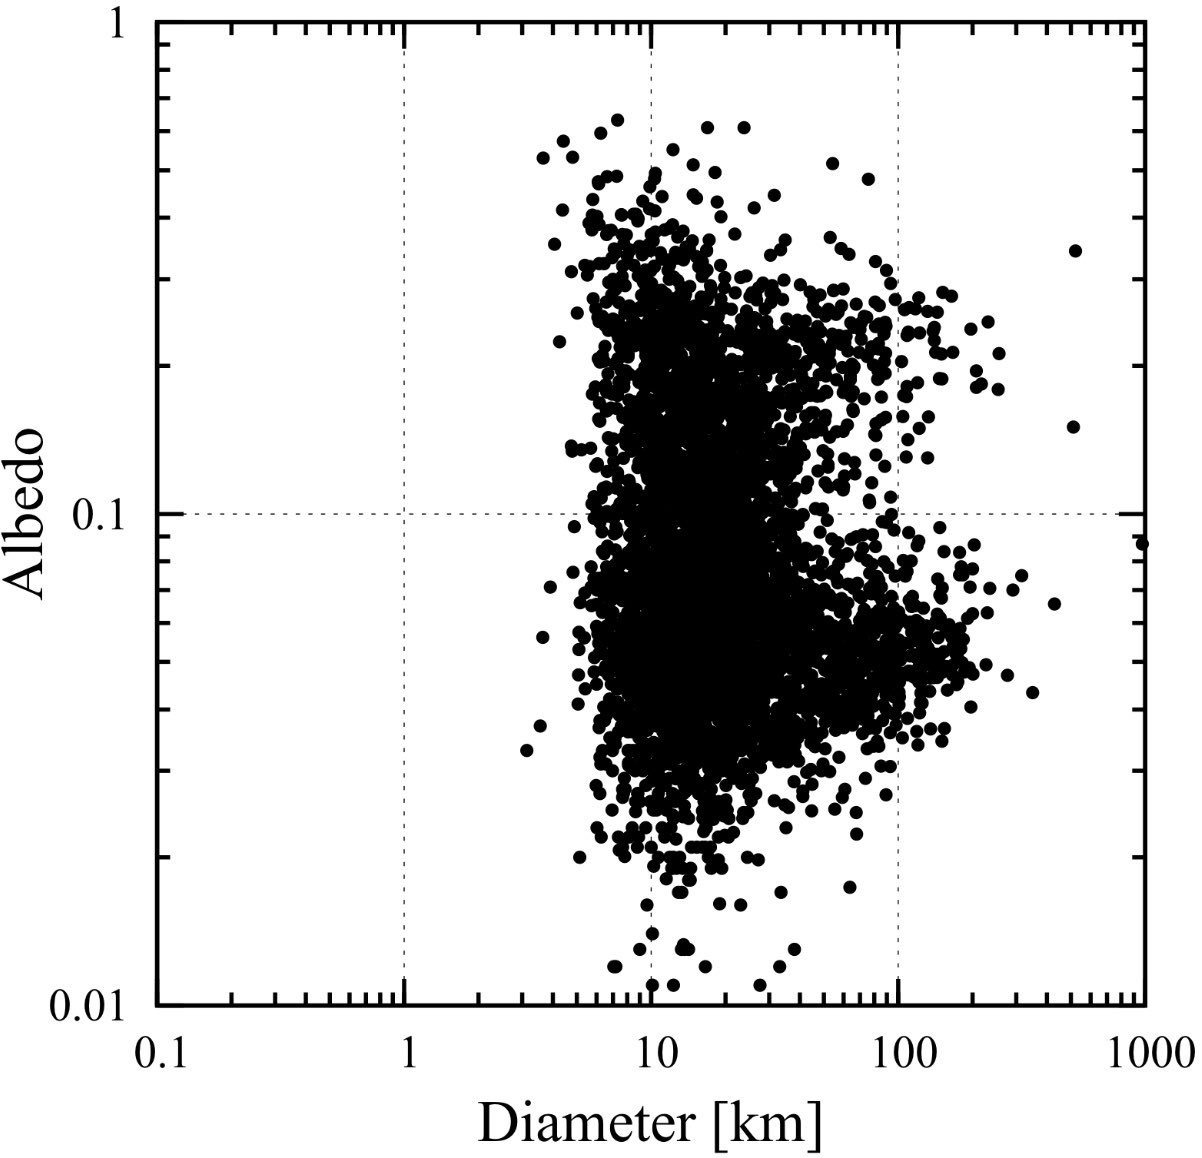
\includegraphics[keepaspectratio,angle=-90,origin=c,width=0.95\textwidth]{A-D}\end{figure}
\begin{block}{Composizione}
Absorption band: silicates, water ices, hydrated minerals.
\end{block}
\end{column} \end{columns}
\begin{block}{Classificazione dinamica}
\begin{itemize}
\item Fascia principale: tra Marte (perielio \SI{1.66}{\astronomicalunit}) e Giove.
\item Rapido spopolamento man mano che ci si avvicina a Giove.
\item Lacune di Kirkwood: per valori del semi-asse maggiore risonanti con quello di Giove.
\item grouping of proper elements: famiglie collisionali
\item Evolution $\tau\si{\mega\year}$: increasing eccentricity cause collision with inner planets or Sun
\end{itemize}
\end{block}
\end{frame}

\begin{wordonframe}{Classificazione asteroidi: orbita, spin, albedo, etc}
Sono la principale sorgente di meteoriti.
Orbite comprese tra Marte e Giove. Il primo \'e 1Ceres, diametro circa \SI{1000}{\kilo\meter}.
Da Terra si vedono come sorgenti puntiformi. Forma, dimensioni e caratteristiche superficiali: tecniche interferometriche e fenomeni di occultamento.
La spettro di riflessione \'e vario: dipende dalle caratteristiche chimiche e fisiche della superficie.
(hydrated minerals includes $H_2O$, $OH$ in crystall structure)
Paucity of asteroid in mean motion/secular resonance with planets.
Disruptive collisions (mean $v_r$ circa 4 $v_e$(ceres)$\approx\SI{5}{\kilo\meter\per\second}$).
Large metallic asteroids: differentiated primordial object stripped of their mantle.
\end{wordonframe}

\begin{frame}{Evoluzione. Kirkwood gap: Resonances in main belt}
\begin{figure}[!ht]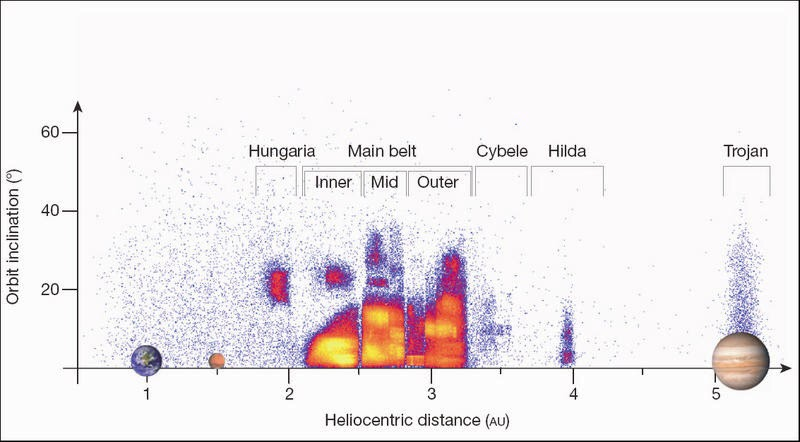
\includegraphics[keepaspectratio,width=0.9\textwidth]{MBplanets}
\end{figure}
\begin{block}{Perturbation}
\begin{itemize}
\item Collisioni: disruptive collisions (truncation at Mars perihelion \SI{1.66}{\astronomicalunit}), inject in resonannt regions, A. families,
\item Resonances: ejection solar system, NEO.
\item Proper elements excitation ($\tau\approx\SIrange{10}{50}{\mega\year}$): $\bar{e}\approx0.13$, $\bar{I}\approx\ang{7}$.
\end{itemize}
\end{block}
\begin{block}{Resonances}
\begin{itemize}
\item 3/1 mean motion resonance with Jupiter (\SI{2.5}{\astronomicalunit}) is instable due to secular resonance: eccentricity increse close to 1 due to collision or Yarkovsky effect
\item First order resonance 2/1, 3/2, 4/3 with J stable: (Z), (H), (T).
\item $\nu_6$ longitude of pericentre drift $\varpi$ drift due to Jupiter perturbation at rate $g_6\approx\SI{28.2}{\arcsecond\per\year}$: truncation at \SI{2.1}{\astronomicalunit} and bent in $(a,I)$ plane.
\end{itemize}
\end{block}
\end{frame}

\begin{wordonframe}{resonances in MB (distribuire)}

$\varpi=\Omega+\omega$: (longitudine del nodo ascendente e argomento del periastro).

In the asteroid belt within 3.5 AU from the Sun, the major mean-motion resonances with Jupiter are locations of gaps in the asteroid distribution, the Kirkwood gaps (most notably at the $3:1$, $5:2$, $7:3$ and $2:1$ resonances).

The perihelion secular resonance between asteroids and Saturn  helps shape the asteroid belt. Asteroids which approach it have their eccentricity slowly increased until they become Mars-crossers, at which point they are usually ejected from the asteroid belt by a close pass to Mars. This resonance forms the inner and "side" boundaries of the asteroid belt around 2 AU, and at inclinations of about $\ang{20}$.

Asteroids have been ejected from these almost empty lanes by repeated perturbations. However, there are still populations of asteroids temporarily present in or near these resonances. For example, asteroids of the Alinda family are in or close to the $3:1$ resonance, with their orbital eccentricity steadily increased by interactions with Jupiter until they eventually have a close encounter with an inner planet that ejects them from the resonance.

A secular resonance occurs when the precession of two orbits is synchronised (usually a precession of the perihelion or ascending node). A small body in secular resonance with a much larger one (e.g. a planet) will precess at the same rate as the large body. Over long times (a million years, or so) a secular resonance will change the eccentricity and inclination of the small body.
\end{wordonframe}

\begin{frame}{famiglie collisionali: grouping in space of proper elements}
\begin{columns}[T]
\begin{column}{0.65\textwidth}
\begin{figure}[!ht]
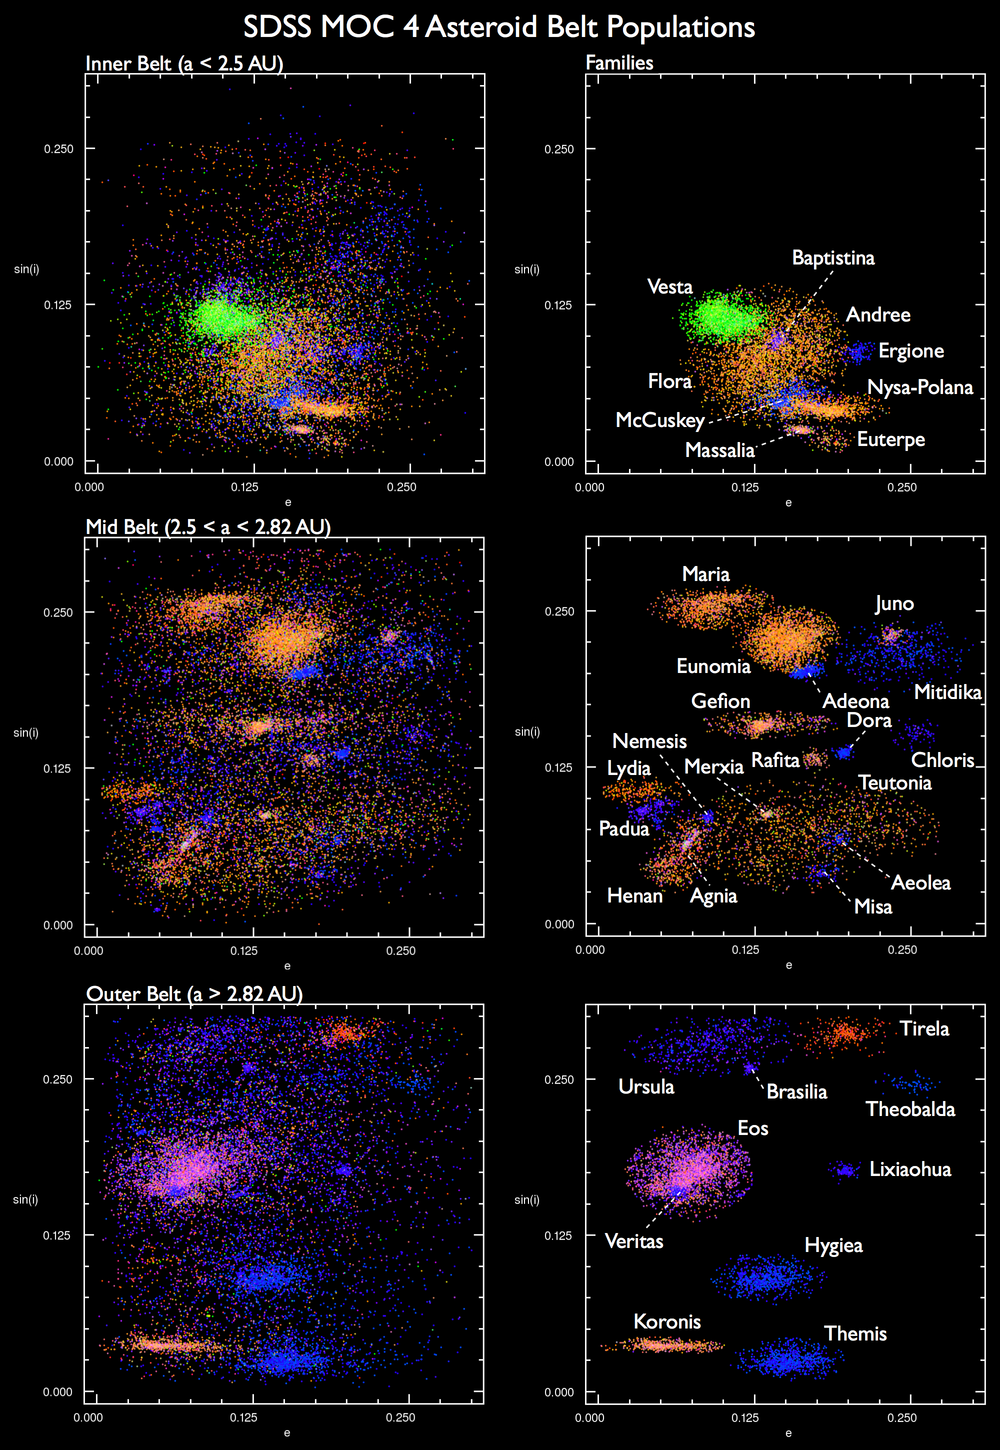
\includegraphics[keepaspectratio,height=0.85\textheight]{Asdss}
\end{figure}
\end{column}
\begin{column}{0.35\textwidth}
Collisional breakup of parent body (Hirayama): velocit\'a relative dei frammenti risultanti molto minori della velocit\'a orbitale.
\begin{block}{Families formation (dynamical aging)}
\begin{itemize}\item Entiere disruption of A. by similar size projectile \item Ejecta from non disruptive collisions (Vesta)
\item oggetti pi\'u grandi sono pi\'u rappresentativi della popolazione iniziale
\end{itemize}
\end{block}
\end{column}
\end{columns}
\end{frame}

\begin{wordonframe}{famiglie collisionali}\tolbf
\begin{block}{Distruptive collisione}
Velocit\'a relativa media \SI{5}{\kilo\meter\per\second} (4 times $v_e$(Ceres))
\end{block}
Most pop. families (similar surface composition): Themis, EOS, Koronis, Vesta. Age: \SIrange{1}{3}{\giga\year}.
\end{wordonframe}

\begin{frame}{Distribuzione di massa degli asteroidi: legge di potenza.}
\begin{block}{Collisional cascade}
\begin{columns}[T]\begin{column}{0.5\textwidth}
Popolazione di asteroidi $N_1$, $N_2$ con $m_1\gg m_2$.
Stato stazionario: $N_1=\gamma N_2$.
\end{column}\begin{column}{0.5\textwidth}
\begin{align*}
&\TDy{t}{N_1}=-\alpha\sigma_1N_1^2\\
&\TDy{t}{N_2}=(-\frac{N_2}{\tau})-\alpha\sigma_2N_1^2+(\frac{m_1}{m_2})\alpha\sigma_1N_1^2
\end{align*}
Sezioni d'urto geometriche: $\sigma_1=\sigma_2(\frac{m_1}{m_2})\expy{\frac{2}{3}}$.
\begin{equation*}
N_2=(\frac{m_1}{m_2})\expy{\frac{5}{6}}N_1
\end{equation*}
\end{column}  \end{columns}
\end{block}
\begin{block}{Legge di potenza alla Dohnanyi}
 Numero di oggetti in $[m,m+dm]$
\begin{equation*}
n(m)\propto m\expy{-\frac{11}{6}}
\end{equation*}
\end{block}
\begin{block}{$\alpha$ osservato}
MB: $\alpha\approx\numrange{1.3}{2}$
Lab.: $\alpha\approx1.8$
Large bodies ($D>\SI{10}{\kilo\meter}$): $\alpha\approx2.1$
NEO: $\alpha\approx1.58$
\end{block}
\end{frame}

\begin{wordonframe}{Distro massa A: legge di potenza.}
\begin{block}{Collisional cascade (Dohnanyi 1969) semplificata}
\begin{itemize}
\item Popolazioni stazionarie
\item Evoluzione collisionale: $\sigma\approx r^2$.
\item scaling ideale: effetto di collisione dipende dai rapporti di massa
\end{itemize}
Popolazione di asteroidi $N_1$, $N_2$ con $m_1\gg m_2$: asteroidi grandi spopolati da collisioni i cui frammenti popolano $N_2$, inoltre $N_2$ sono spopolati da collisioni e processo dinamico ($\tau$).
Stato stazionario: $N_1=\gamma N_2$, se $q=\frac{m_2}{m_1}\ll1$ $\gamma=-\frac{q}{2}+\sqrt{(\frac{q}{2})^2+q\expy{\frac{5}{3}}}$.
\end{block}
\end{wordonframe}

\begin{frame}{Size distribution}
\begin{block}{Size distro}
\begin{figure}[!ht]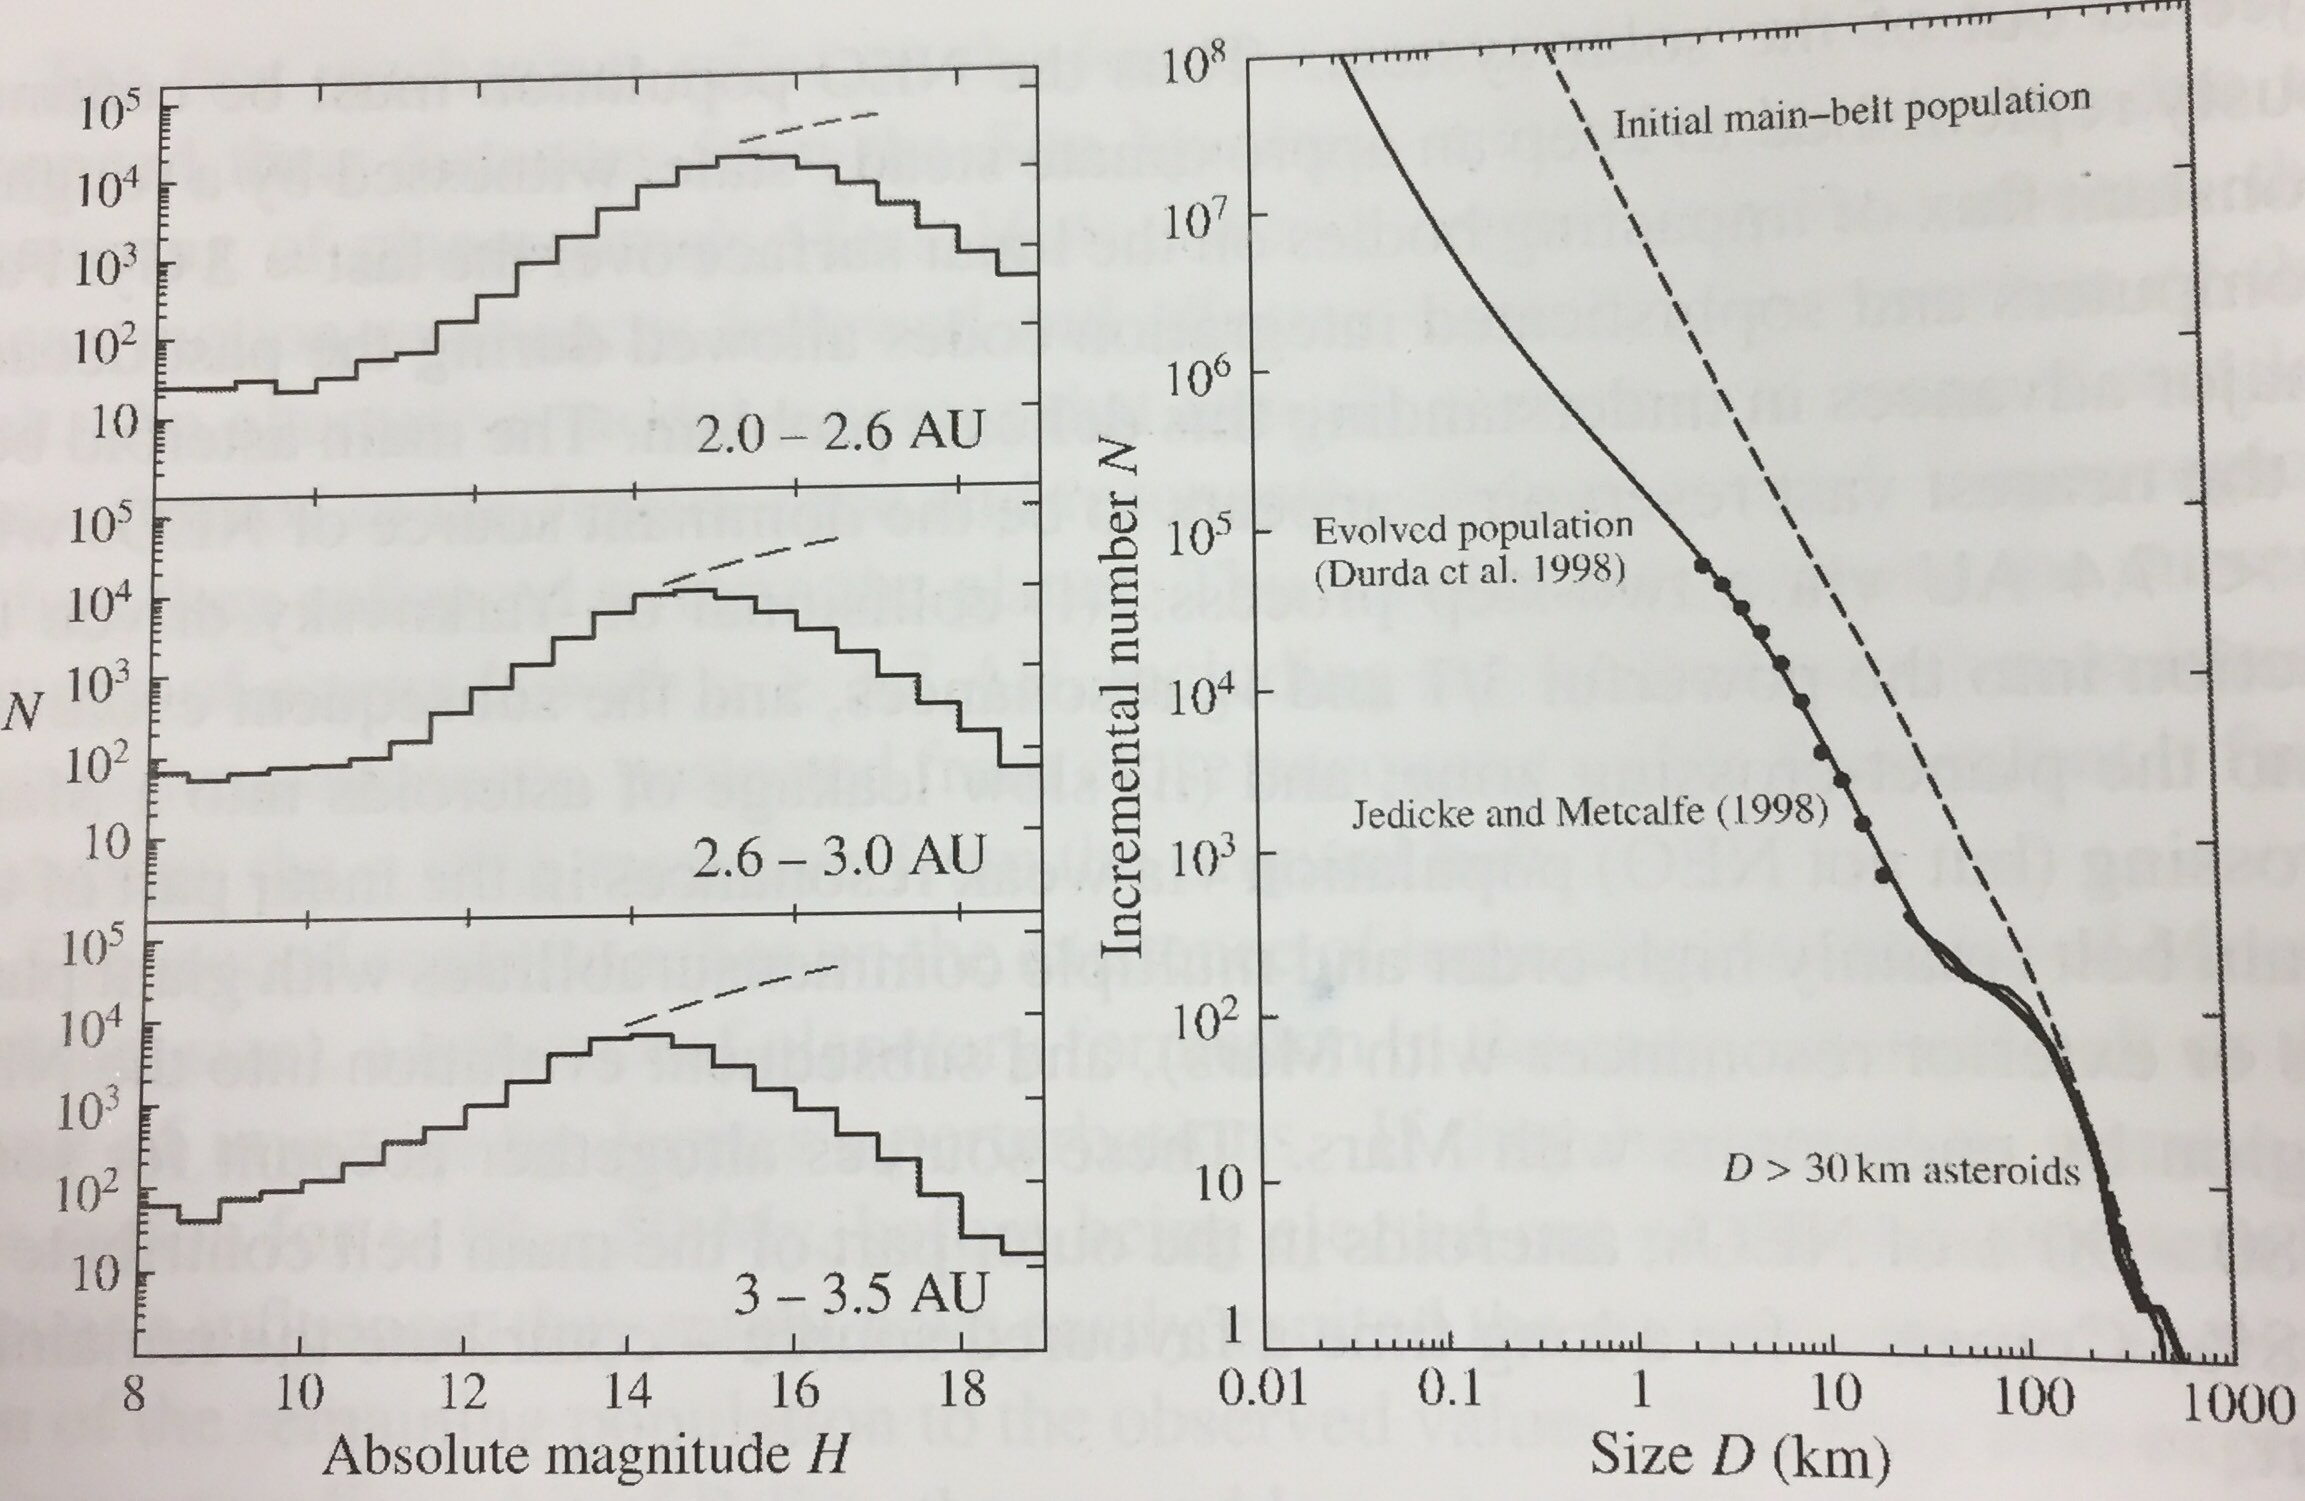
\includegraphics[keepaspectratio,width=\textwidth]{Asizedistro}
\end{figure}
\end{block}
\end{frame}

\begin{wordonframe}{Distribuzione di massa A.}
Most of A mass lies in largest bodies. Excess of bodies around \SI{100}{\kilo\meter}: self-gravitation becomes important at this size for reaccumulation
Distribuzione alla Dohnanyi  $dN\propto m\expy{-\alpha}\,dm\propto D\expy{\beta}\,dD$ (MB:$q<2$)
\end{wordonframe}

\begin{frame}{Depletion of primordial MB}
\begin{columns}[T]\begin{column}{0.5\textwidth}
\begin{itemize}
\item Sweeping mean motion resonances with Jupiter
\item Scattering action of massive planetesimal: left-over of planetary formation or injection by Jupiter perturbation.
\end{itemize}
\end{column}\begin{column}{0.5\textwidth}
\begin{itemize}
\item Effects due to Saturn/Jupiter migration
\item Cluster of core in Jupiter region: depletion of region with $a>\SI{3.3}{\astronomicalunit}$
\end{itemize}
\end{column}\end{columns}
\end{frame}

\begin{frame}{Spin rate}
\begin{columns}[T]
\begin{column}{0.5\textwidth}
\begin{figure}[!ht]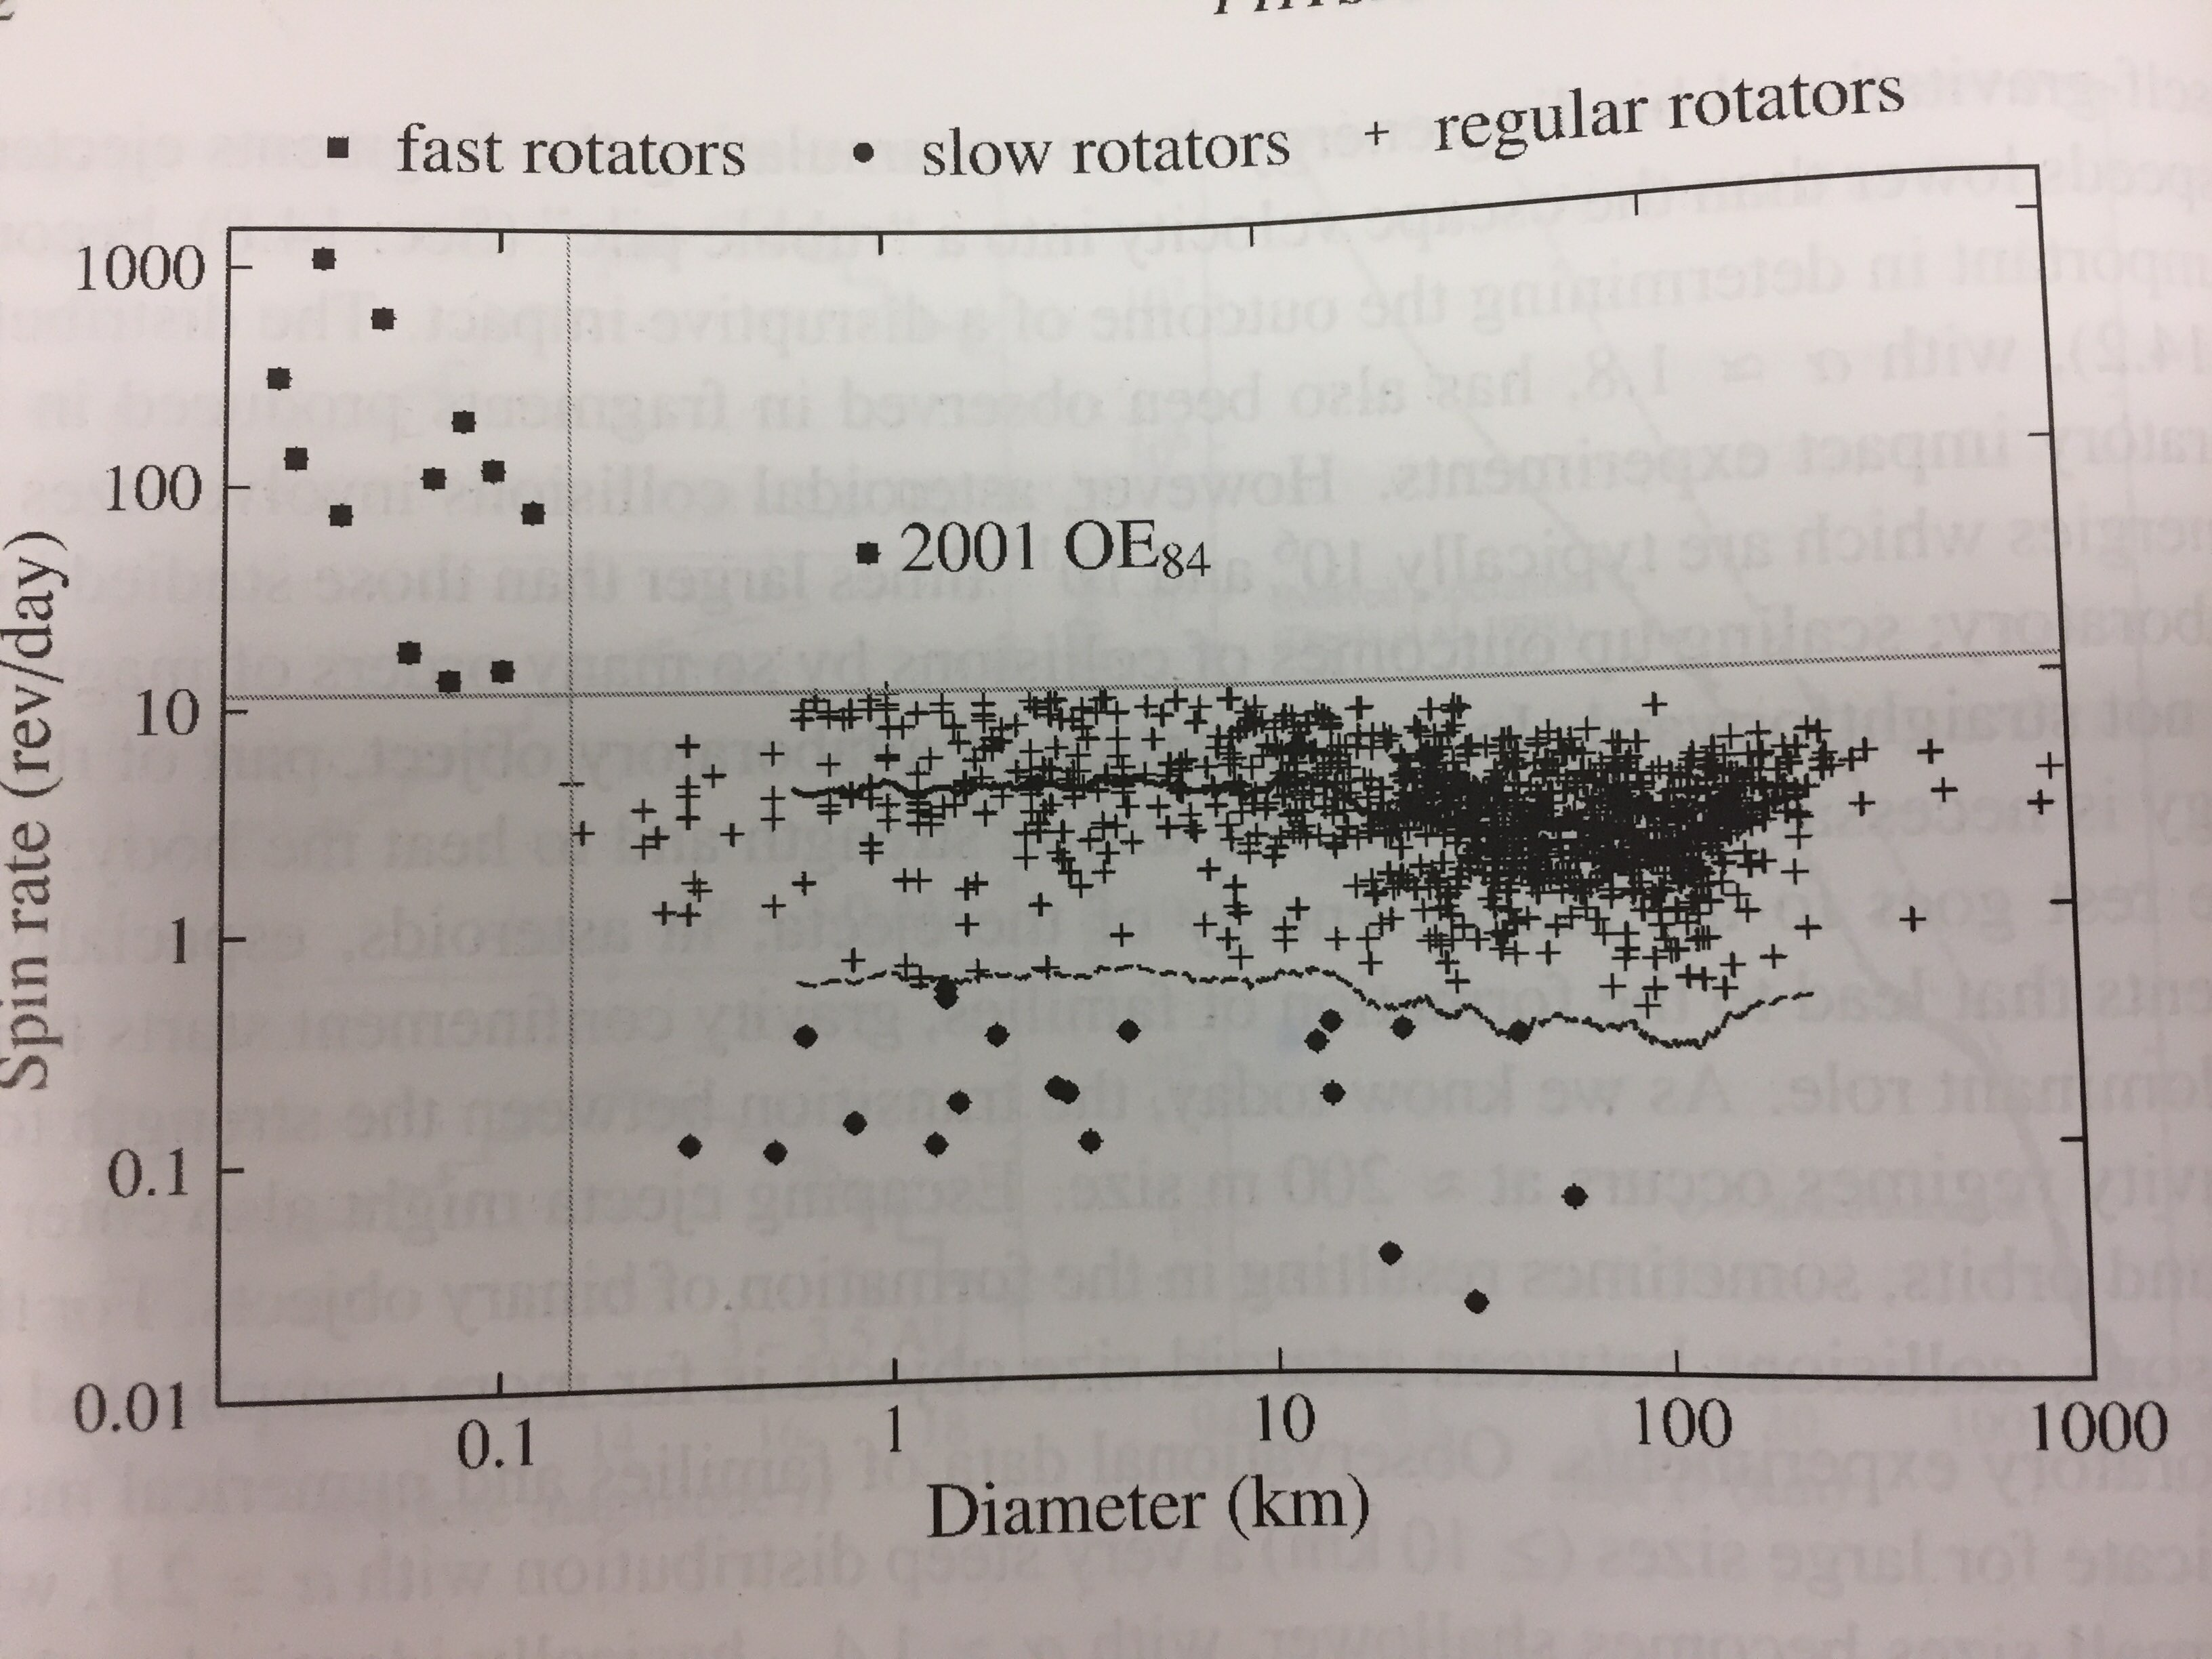
\includegraphics[keepaspectratio,width=0.99\textwidth]{spinD}
\end{figure}
Angular momentum changed by collision and dynamical processes.
\end{column}
\begin{column}{0.5\textwidth}
\begin{itemize}
\item Slow/Fast rotator: $\omega_{cr}\approx\SI{2.1}{\hour}$ (vanishing strength, $\bar{\rho}=\SI{2.5}{\gram\per\cubic\cm}$).
\end{itemize}
\begin{block}{Slow rotator}
Braking: loss of close satellite, radiation torque (smaller)
\end{block}
\begin{block}{Binary Asteroid}
\begin{itemize}\item $20\%$ NEO
\item Small eccentricity of rel. motion
\item Formation: tidal fission, capture of ejecta
\end{itemize}
\end{block}
\end{column}
\end{columns}
\end{frame}

\begin{wordonframe}{Asteroid spin}

\end{wordonframe}

\subsection{NEO/NEA and meteorites}\linkdest{NE}

\begin{frame}{NEO - NEA}
a: \SIrange{1.3}{0.983}{\astronomicalunit}. Ganymede(Amor)$\approx\SI{38.5}{\kilo\meter}$.
$\tau_{NEO}\approx\SI{10}{\mega\year}$.
Constant flux of impacting bodies on the Moon over \SI{3}{\giga\year}.
\begin{block}{NEA/O sources}
\begin{itemize}
\item Yarkovsky -> 3/1,$\nu_6$ resonances
\item MB->Mars crossing(WR)
\item Outer MB
\item Comets
\end{itemize}
\end{block}
Space weathering: esposizione superficie a meteoriti, radiazione, vento solare.
\begin{block}{Caratteristiche fotometriche}\end{block}
\end{frame}

\begin{wordonframe}{Neo e Nea}
Orbita pi\'u interna, incrocia anche l'orbita della Terra. Apollos/Atens can hit the Earth, Amor can only approach but planetary perturbation can bring it into collisional orbit in \SIrange{e3}{e5}{\year}. 
\end{wordonframe}

\begin{frame}{Meteoriti}
\begin{figure}[!ht]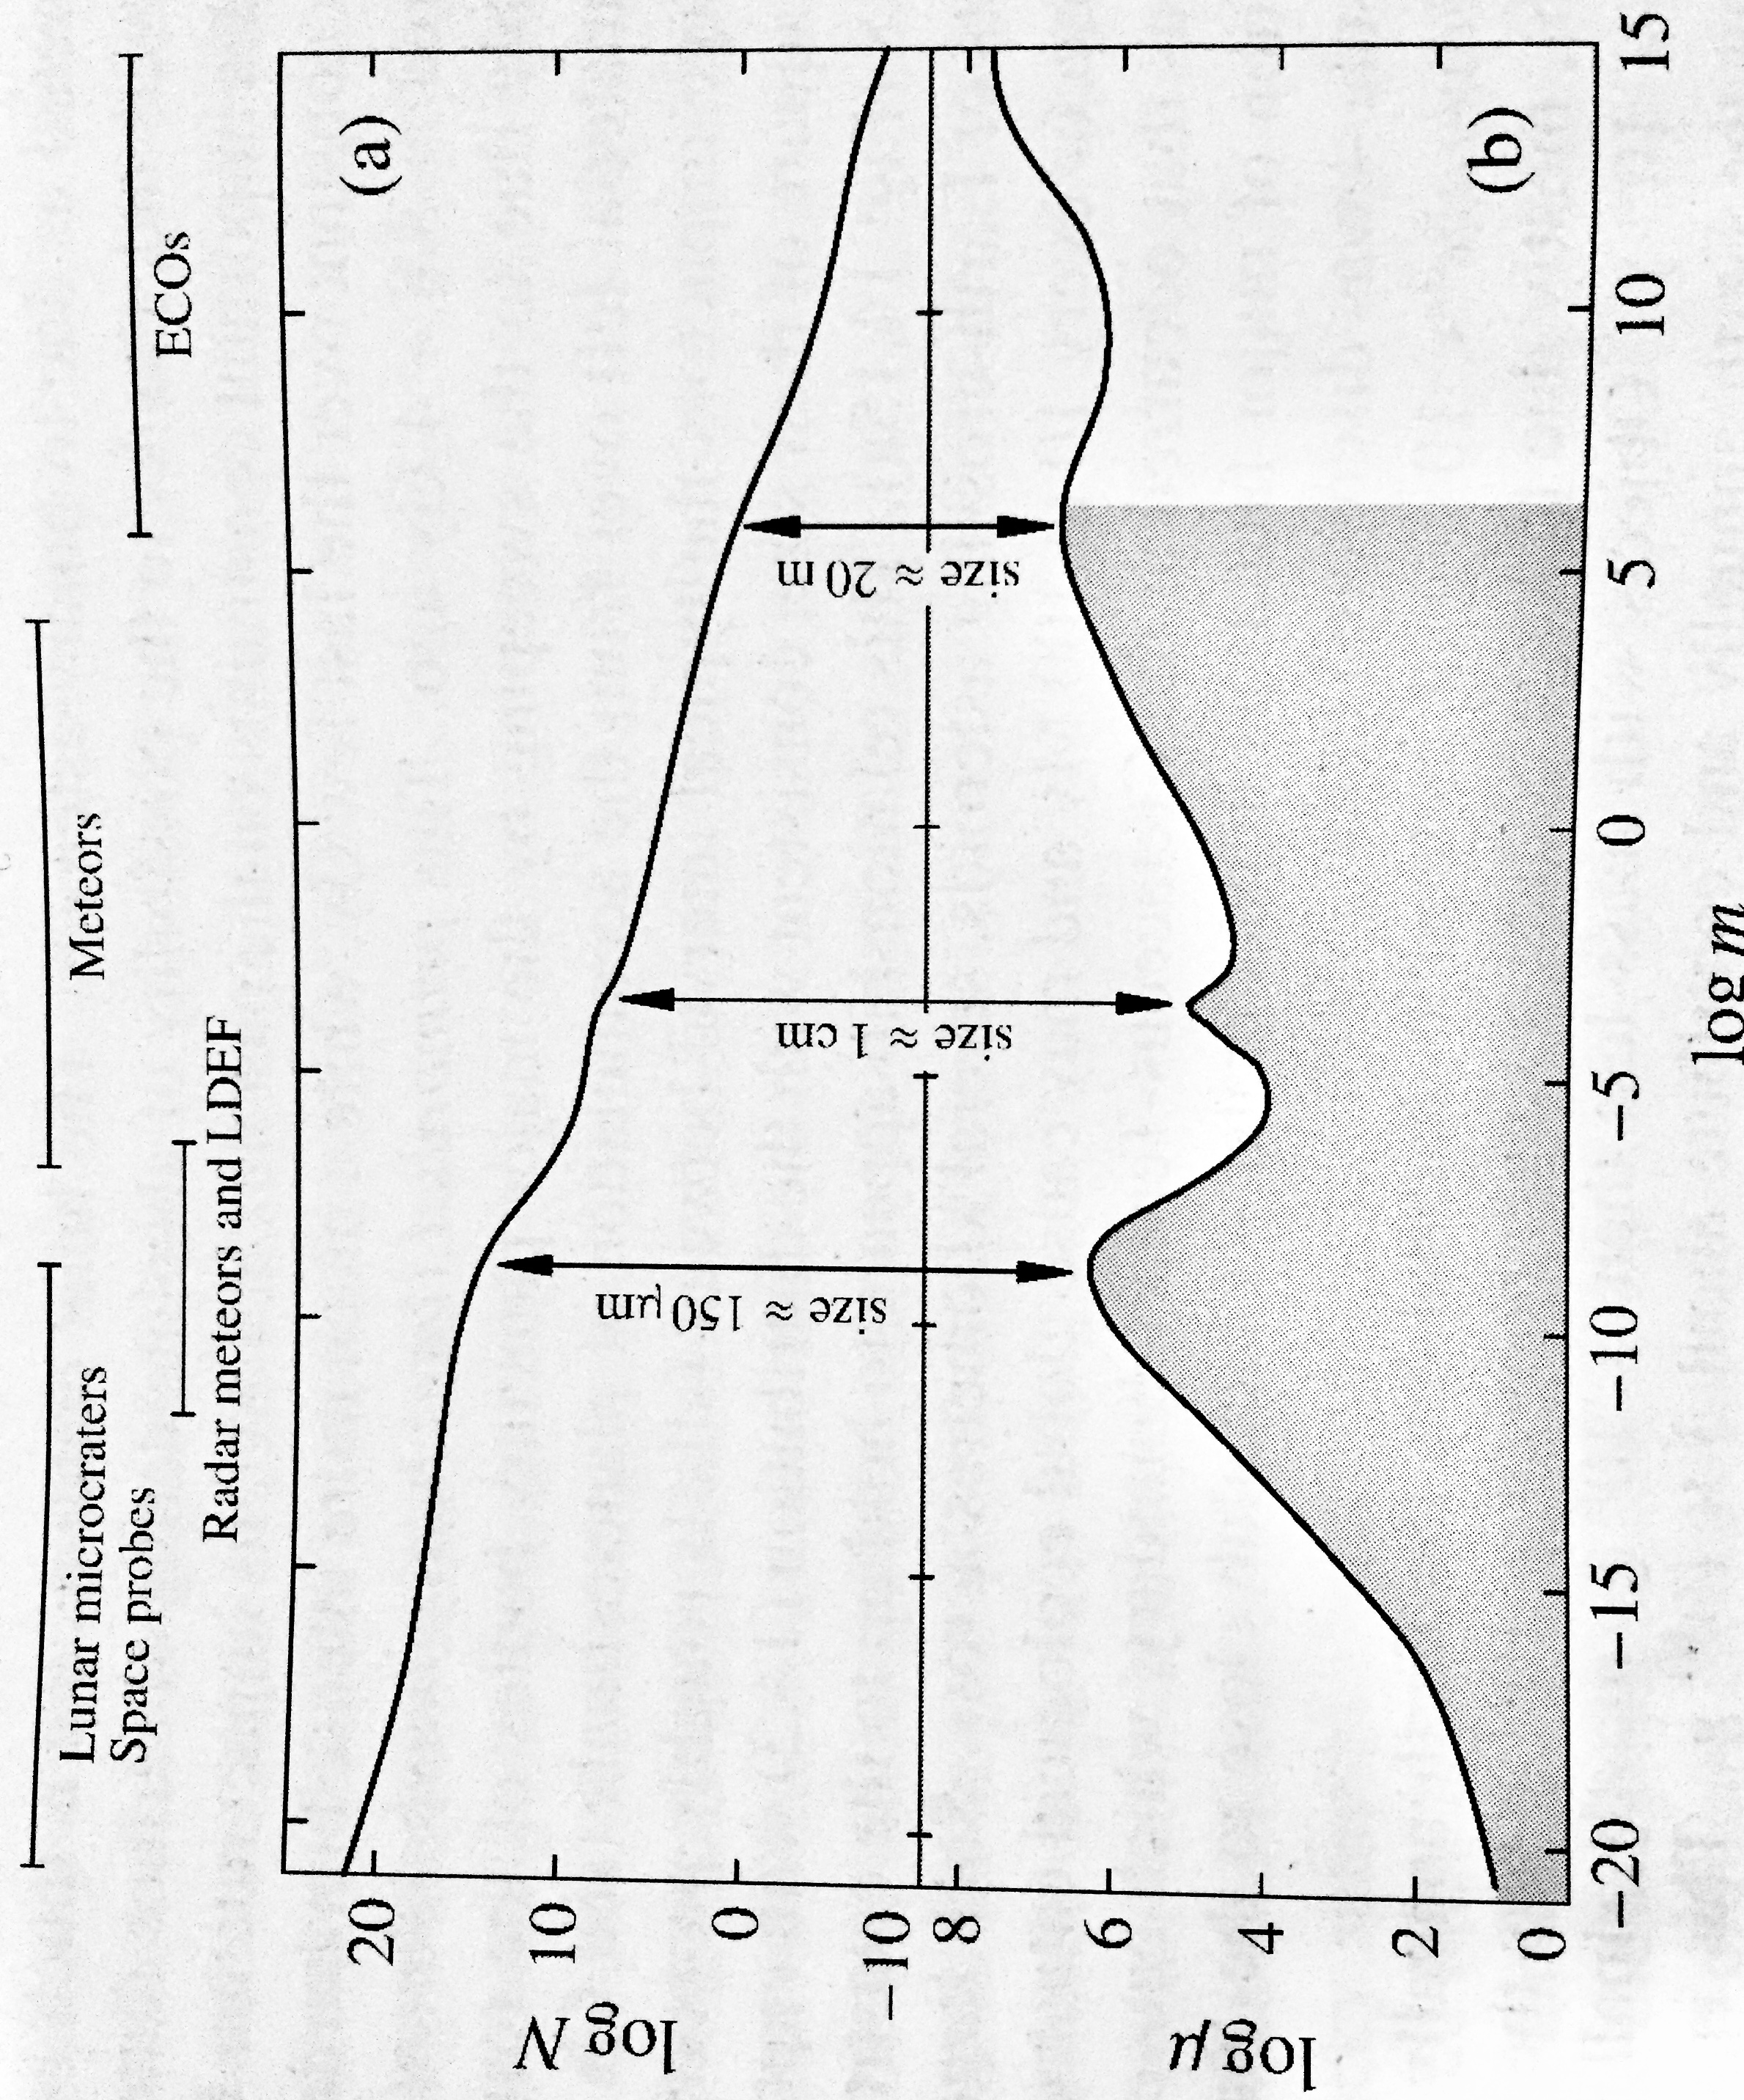
\includegraphics[angle=-90,keepaspectratio,width=\textwidth]{meteorites}\end{figure}
\begin{itemize}
\item Dust band at $I=\pm\deg{2},\pm\deg{10}$ (Inclination of 3 most populated A. families)
\end{itemize}
\begin{block}{Timescale}
\begin{itemize}
\item Crystallization age
\item Cosmic ray exposure age
\item Terrestrial age
\end{itemize}
\end{block}
\end{frame}

\begin{wordonframe}{meteoriti}
$N(m)$ numero oggetti con massa minore di m e $\mu(m)$ is total mass of those object.
\end{wordonframe}

\subsection{Satelliti e anelli}\linkdest{satrings}

\begin{frame}{Caratteristiche anelli planetarii}
\begin{itemize}
\item Flatness on equatorial plane: rings settle in equatorial plane in $\frac{1}{\nu_c}\approx \frac{1}{\Omega\tau}$.
\item Larghezza $\approx R_p\approx\rroc{}$
\item 
\end{itemize}
\end{frame}

\begin{wordonframe}{Teoria anelli}
\begin{columns}\begin{column}{0.5\textwidth}
Gas kinetic: $\exv{v^2}=\frac{KT}{\mu m_p}$ ($\\frac{1}{2}m\exv{v^2}=\frac{f}{2}KT$)
\end{column} \begin{column}{0.5\textwidth}
Optical properties: $\tau\approx nSH=n_p\sigma H$
\end{column}  \end{columns}
\end{wordonframe}

\begin{frame}{Modello di anello freddo}
\begin{align*}
&m_r=2\pi\rho H\delta r(r_0+\delta r/2)\\
&L=\int\,dm\sqrt{GM_p}r\expy{1/2}=\sqrt{GM_p}2\pi\rho H\int r\expy{3/2}\,dr\\
&E=-\frac{1}{2}GM_p\int \frac{dm}{r}=GM_p\pi\rho H \delta r
\end{align*}
Concentro tutta la massa a una distanza data. Conservazione energia determina un raggio $R_E$, conservazione momento angolare $R_L$:
\begin{align*}
&\frac{R_L}{R_E}\approx1+(\frac{\delta r}{4r_0})^2\\
&\Delta E\approx -\frac{GM_p_r}{r}[(\frac{\delta r}{4r})^2_f-(\frac{\delta r}{4r})^2_i]\approx\frac{GM_p_r}{r}(\frac{\delta r}{4r})^2_i\\
&\Delta E_{grav}\approx\frac{Gm_r^2}{r}
\end{align*}
Per stringer l'anello: $\Delta E_{grav}\geq\Delta E$ cio\'e $\frac{m_r}{M_p}\geq(\frac{\delta r}{4r})^2$.
Un anello stretto: giovane o massiccio o tenuto stretto da altro effetto.
\end{frame}

\begin{wordonframe}{Anello dominato da evoluzione collisionale - freddo - sottile}
Teorema viriale: $\exv{E}=\frac{1}{2}\exv{U}$.
\end{wordonframe}

\begin{frame}{Anelli di Saturno}
Refs - Goldreich tremaine: Dynamics planetary rings'' (pg4),  
\end{frame}

\subsection{Kuiper, TNO, comete.}\linkdest{Ktnocs}

\begin{frame}{Reservoir di corpi}

\end{frame}

\begin{wordonframe}{Jupiter class comets}

\end{wordonframe}

\begin{frame}{Resonanze in TNO}
The orbits of Pluto and the plutinos are stable, despite crossing that of the much larger Neptune, because they are in a 2:3 resonance with it.
In the rings of Saturn, the Cassini Division is a gap between the inner B Ring and the outer A Ring that has been cleared by a $2:1$ resonance with the moon Mimas. (More specifically, the site of the resonance is the Huygens Gap, which bounds the outer edge of the B Ring.)
    In the rings of Saturn, the Encke and Keeler gaps within the A Ring are cleared by 1:1 resonances with the embedded moonlets Pan and Daphnis, respectively. The A Ring's outer edge is maintained by a destabilizing $7:6$ resonance with the moon Janus.
Most bodies that are in resonance orbit in the same direction; however, a few retrograde damocloids have been found that are temporarily captured in mean-motion resonance with Jupiter or Saturn. Such orbital interactions are weaker than the corresponding interactions between bodies orbiting in the same direction.
\end{frame}

\begin{frame}{Troiani e centauri.}
Troiani: sono oggetti che hanno lo stesso semi-asse di Giove ma spostati di \ang{+-60} nell'orbita cio\'e nei punti Lagrangiani.
Centauri: orbite comprese tra Giove e Nettuno. La zona \'e dinamicamente instabile e porta in orbite cometaria.
\end{frame}

\begin{frame}{Trans-Neptunian object: Fascia di Kuiper-Edgeworth.}
Oltre Nettuno di hanno i TNO.
Un sottogruppo dei TNO, i plutini, sono in risonanza $3:2$ con Nettuno (come Plutone).
\end{frame}

\begin{frame}{Comete}
Orbite eccentriche.

Il cambiamento delle loro propriet\'a dipende dalla distanza dal Sole: ricche di sostanze volatili

Originaria di una fascia esterna di corpi minori compresa tra asteroidi e TNO, in seguito a incontri ravvicinati con corpi maggiori si sono spostate in orbite che raggiungono all'afelio i confini del sistema solare (Nube di Oort approx \SI{e5}{\astronomicalunit}: quando diventa prevalente l'attrazione delle stelle vicine).
\end{frame}

\begin{frame}{Search motivation}
\begin{itemize}
\item Why acretional formation of solar system planet objects should stop at Neptuno's distance.
\item The jupiter family comets are almost on planar orbits with low inclination on ecliptic plane (plane of solar system). This is inesplicable if the source is far away and isotropic, so we may may postulate a a disc of cometary object beyond Neptun.
\end{itemize}
\end{frame}



\part{Sistemi extra-solari.}\linkdest{exosystem}

\begin{frame}{this part toc}
\begin{itemize}
\item Caratteristiche sistemi extra-solari
\item Pianeti abitabili
\end{itemize}
\end{frame}

\section{extrasolar: todo}

\begin{wordonframe}{Osservazioni: Da ''Physical properties of extrasolar planets''}\tolbf
\begin{itemize}
\item Observed properties: ralation host star metallicity-frequency pf planets, large radius of transiting planets; pg 42 radius anomaly, brown dwarf vs massive planets, Hot Neptune (link to seminario?), light from exoplanets.
\item Interior structure: pg13 EOS composition, Earth-super Earth and Neptune-Super jupiter (18-19); Evolution (pg 30)
\end{itemize}
\end{wordonframe}

\begin{wordonframe}{Udry 03:I, II}
constrain on migration scenario: runaway migration
\end{wordonframe}

\section{Osservazioni}

\begin{wordonframe}{extrasolar: problemi aperti}
Distinzione pianeta/brown dwarf: $M_P\leq20M_J$, i pianeti veri e propri hanno masse $M_P\leq13M_J$.
Domande fondamentali:
\begin{itemize}
    \item Quanto \'e frequente la formazione di sistemi planetari all'atto di formazione stellare?
    \item Quanto \'e frequente la formazione di pianeti terrestri?
    \item Quanto \'e frequente la nascita della vita?
\end{itemize}
\end{wordonframe}

\begin{frame}[allowframebreaks]{Survey}
\begin{columns}[T]\begin{column}{0.5\textwidth}
\begin{block}{RV}
\begin{itemize}
\item Keck: Cumming 08 ($P<2000d$, $m>0.3\mjupiter$) - Keck and Lick: Howard 10
\item California planet survey (exoplanets.org)
\item HARPS (mayor 11)
\end{itemize}
\end{block}
\end{column}\begin{column}{0.5\textwidth}
\begin{itemize}
\item Corot (Moutou 13)
\item Kepler (kelper-california survey II, III, V, planet occurrence within 0.25 AU, taloe of evaporation): Coughlin 16
\end{itemize}
\end{column}\end{columns}
\begin{itemize}
\item Direct imaging: Bowler 16.
\item Microlensing: cassan 12
\end{itemize}
\begin{block}{Exoplanets catalog}
\begin{itemize}
\item Extrasolar planet encyclopedia: exoplanet.eu
\item Keck, lick, Anglo-Australian telescope: exoplanets.org
\item www.inscience.ch/transits: transit references
nsted.ipac.caltech.edu: nasa planet finding and characterization activities 
\end{itemize}
\end{block}
\end{frame}

\section{Properties of radial velocity exoplanets}
%
\begin{wordonframe}{Revs about stat properties of rv exo}
Udry 03, Udry Santos 07, Santos 08, Johnson 09, Mayor 11 Winn Fabrycky 15, Cumming 14
\end{wordonframe}

\begin{frame}{Fraction of stars with orbiting planets. Detectability in M-P diagram.}

\begin{figure}[!ht]
\begin{subfigure}[b]{0.47\textwidth}
\centering
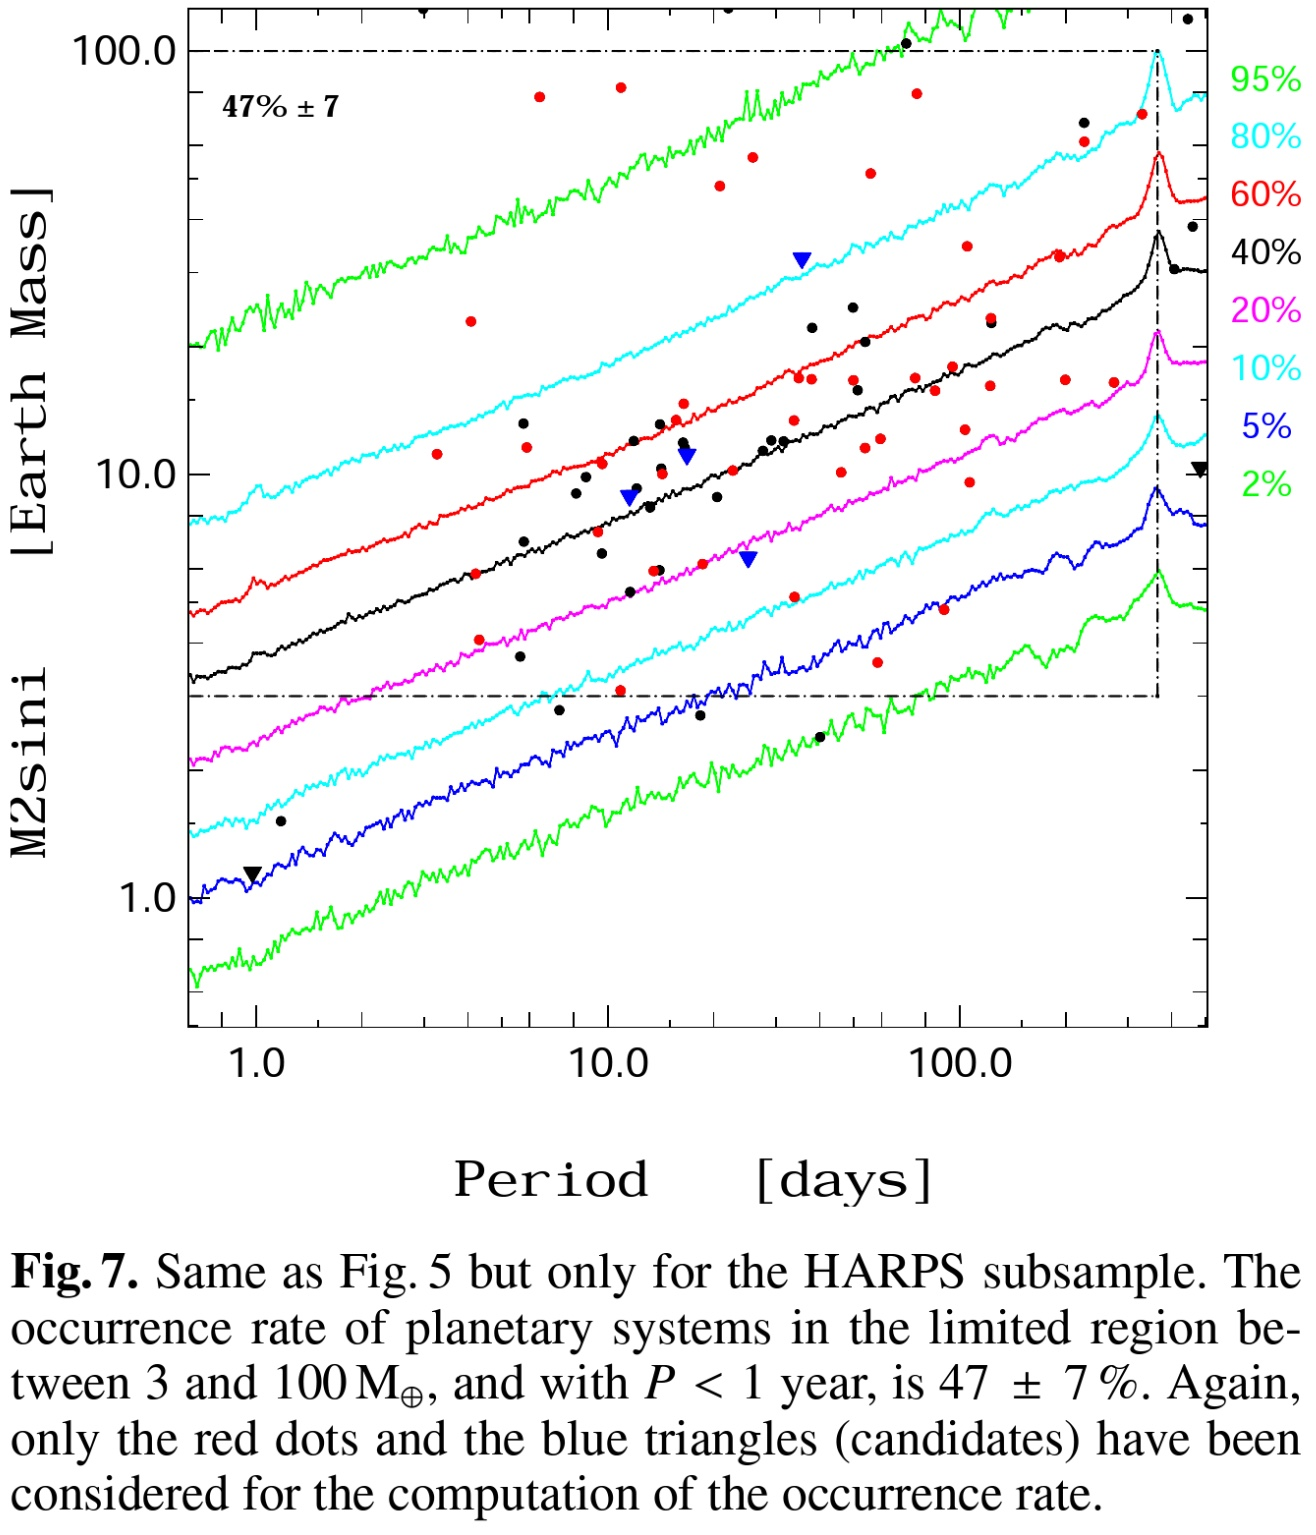
\includegraphics[trim={0cm 0 1 0},clip, keepaspectratio, height=0.4\textheight]{PMfreq-e12}
\label{fig:PMfreq-e12}
\end{subfigure} 
~
\begin{subfigure}[b]{0.47\textwidth}
\centering
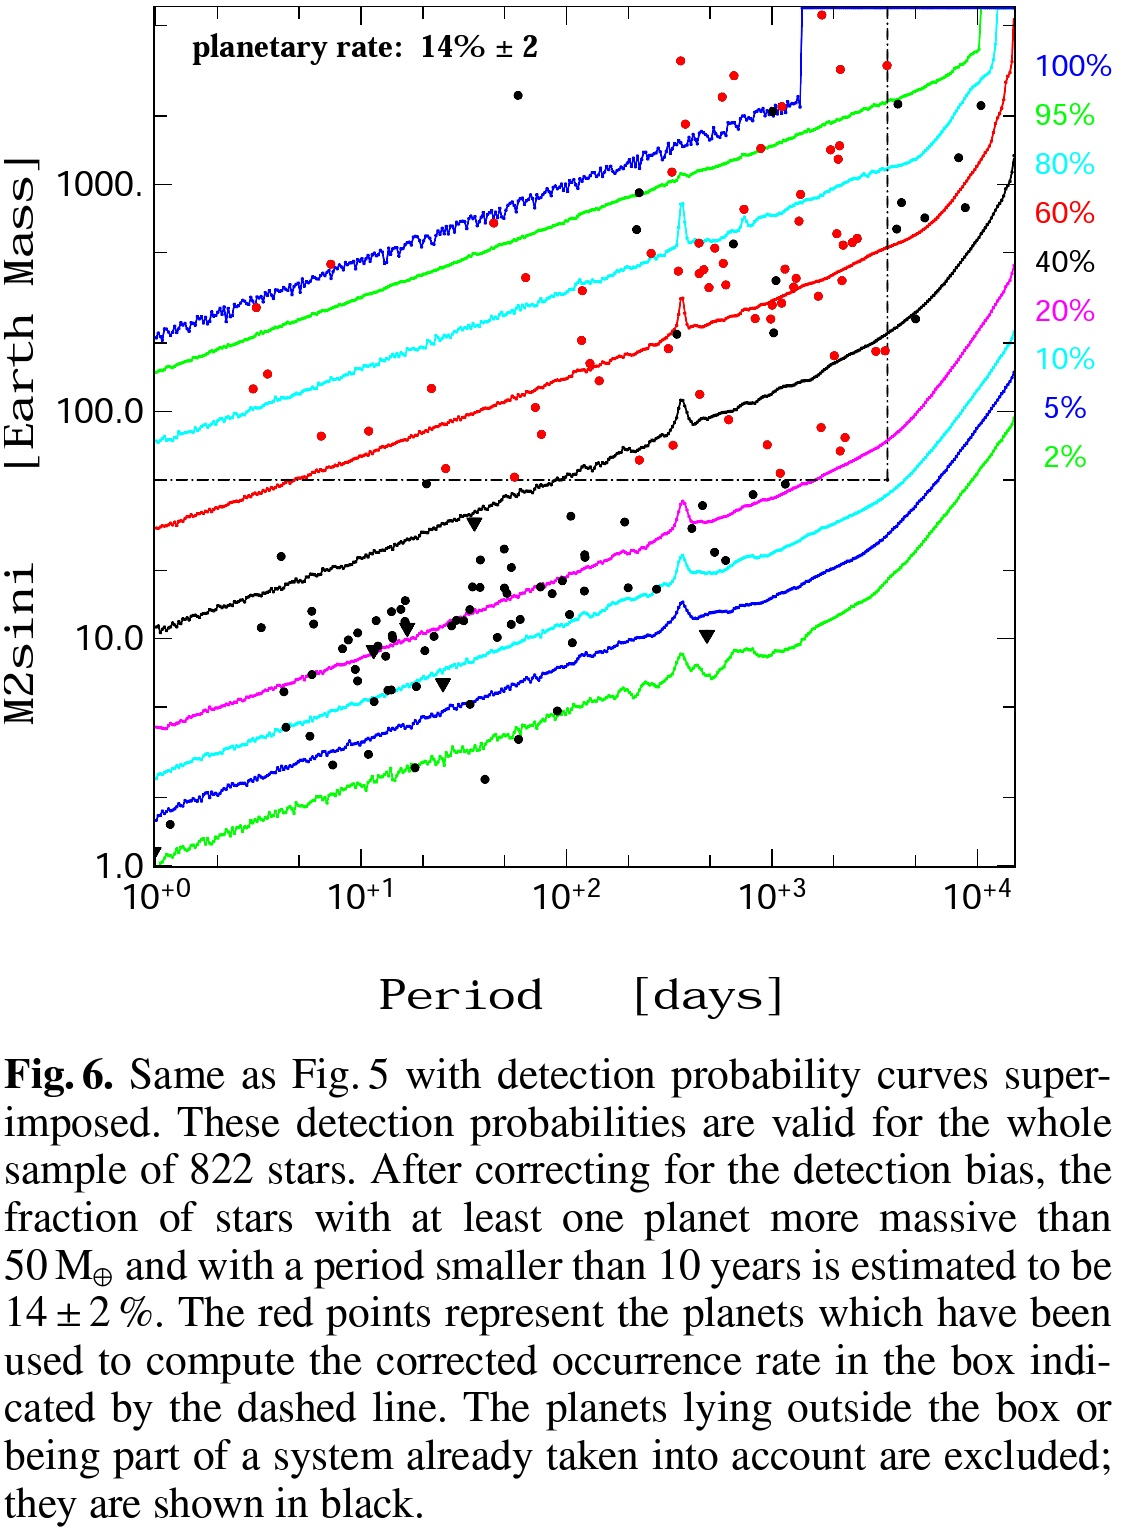
\includegraphics[trim={0cm 0 1 0},clip, keepaspectratio, height=0.4\textheight]{PMfreq-e23}
\label{fig:PMfreq-e23}
\end{subfigure}

\end{figure} 

\begin{figure}[!ht]
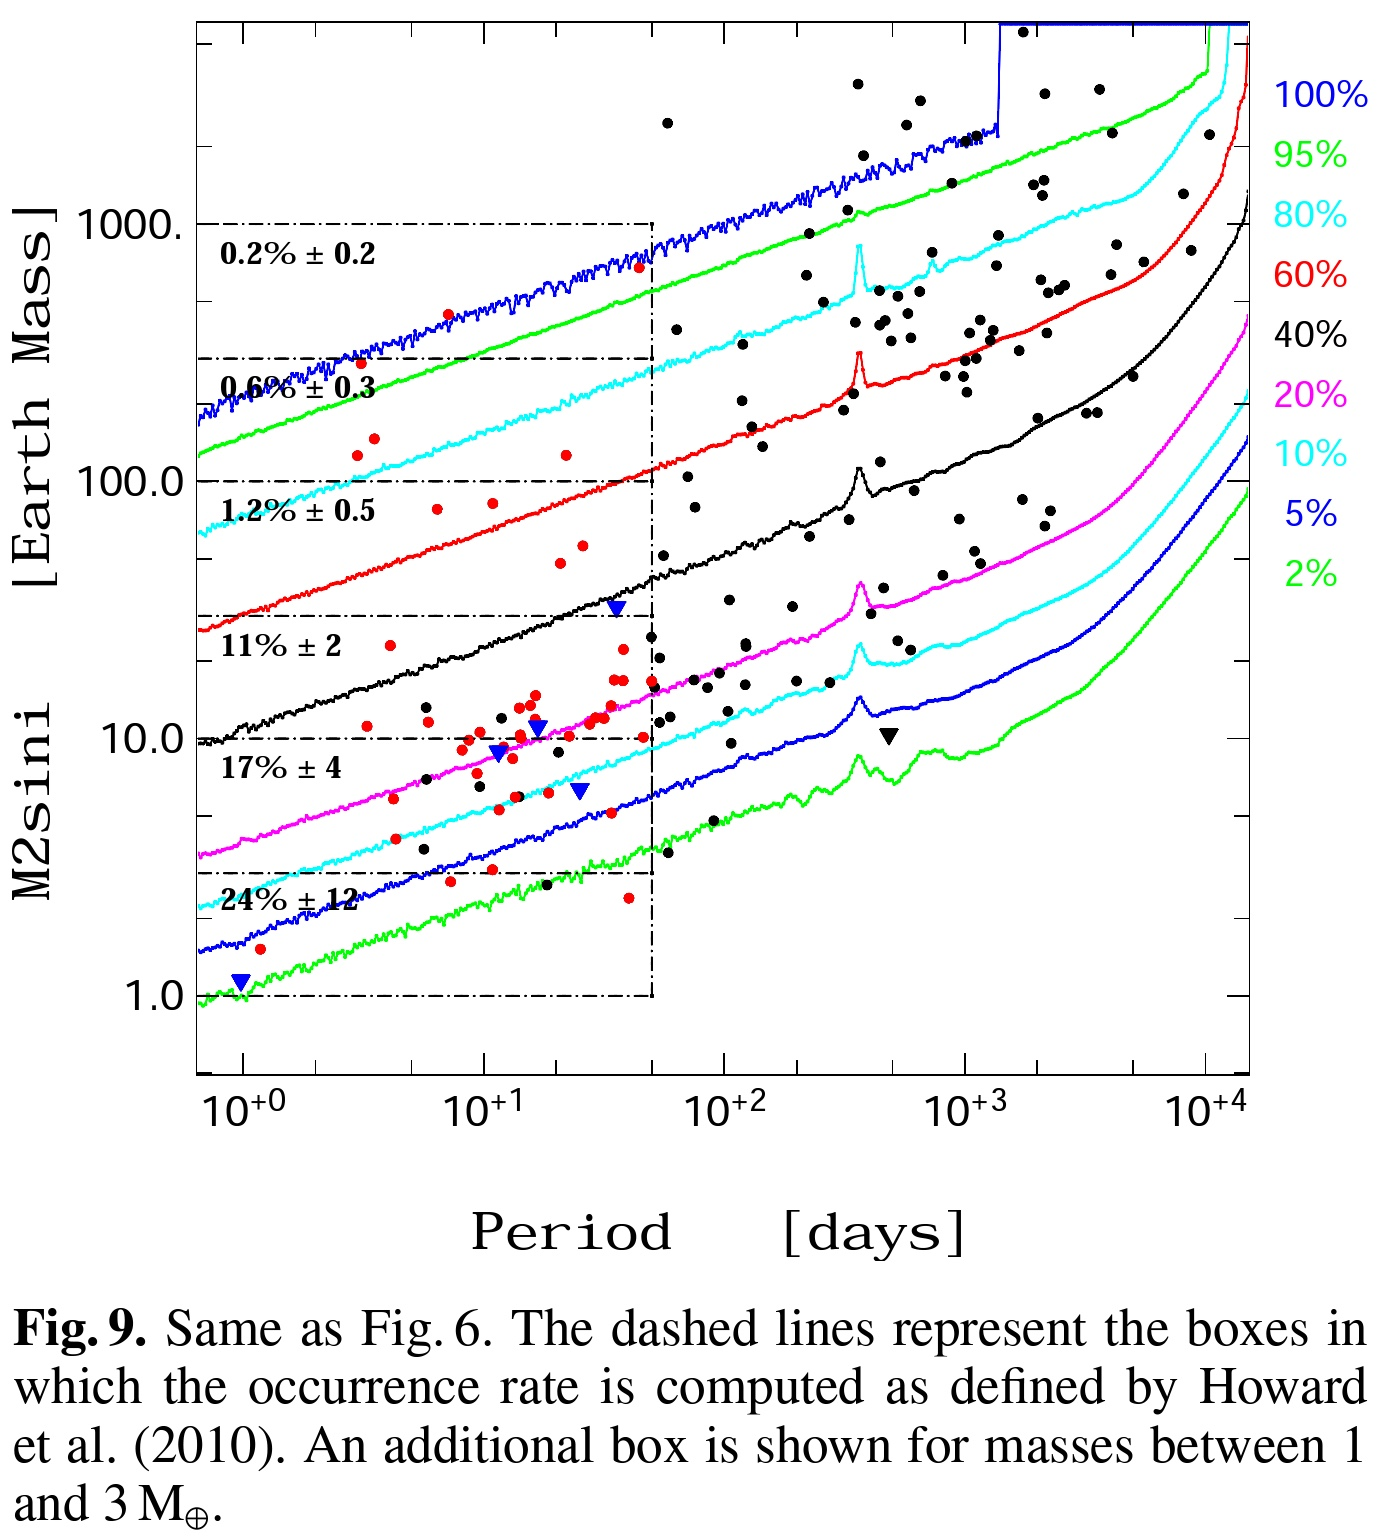
\includegraphics[trim={0cm 0cm 1 0},clip, keepaspectratio,height=0.4\textheight]{PMfreqshort}
\label{fig:PMfreqshort}
\end{figure}

\end{frame}

\begin{wordonframe}{Distribuzioni pianeti osservati tramite RV e completezza survey nello spazio dei parametri M-P}
Le linee colorate nel diagramma massa-periodo delimitano regioni al di sotto delle quali la percentuale indicata ($C(M\sin{i},P)$) di stelle ha $99\%$ di probabilit\'a di rilevamento per un pianeta in quella regione del diagramma.
Il $47\%$ di stelle ospita un pianeta nel range di massa $2\mearth{}-50\mearth{}$ delle super-terre e pianeti gioviani entro $100\mearth{}$, il $14\%$ ha pianeti gioviani ($M_p>50\mearth{}$), il $24\%$, $17\%$ e $11\%$ risp. hanno pianeta terrestre, super-terra e nettuniano con periodo entro $50d$.

$f_{pl}=\frac{1}{N_*}\sum_iN_{ij}$, $N_{ij}=\frac{1}{C(m\sin{i},P)}$ per pianeta i attorno a stella j.
\end{wordonframe}

\begin{frame}{Mass-Period distribution}
\begin{itemize}
\item \cite{marcy2008exoplanet}: Pianeti nel range di massa $0.1-12\mjupiter$ hanno distribuzione di massa $\TDy{M}{N}\propto M\expy{-1.15}$.
\item \cite{cumming2008keck}: nell'intervallo $M=0.3-10\mjupiter{}$ e $P=2-2000\si{\day}$ la distribuzione dei pianeti nel diagramma M-P segue $dn\propto M\expy{\alpha}P\expy{\beta}\,d\log{M}d\log{P}$ con $\alpha=-0.31\pm0.2$, $\beta=0.26\pm0.1$.
\item \cite{mayor2011harps}: $P<\SI{100}{d}$ dominano super-terre e pianeti nettuniani, shortage of massive planets at short periods ($0.5-1\%$ Hot Jupiters), frequency of gaseus giant planets strongly increasing with $\log{P}$, lack of light planet ($M<0.75\mjupiter{}$) on periods larger than \SI{100}{day}.
\end{itemize}
\end{frame}

\begin{frame}{Distribuzione di massa planetaria: RV, Mayor 11}
\begin{figure}[!ht] \begin{subfigure}[b]{0.47\textwidth}
\centering 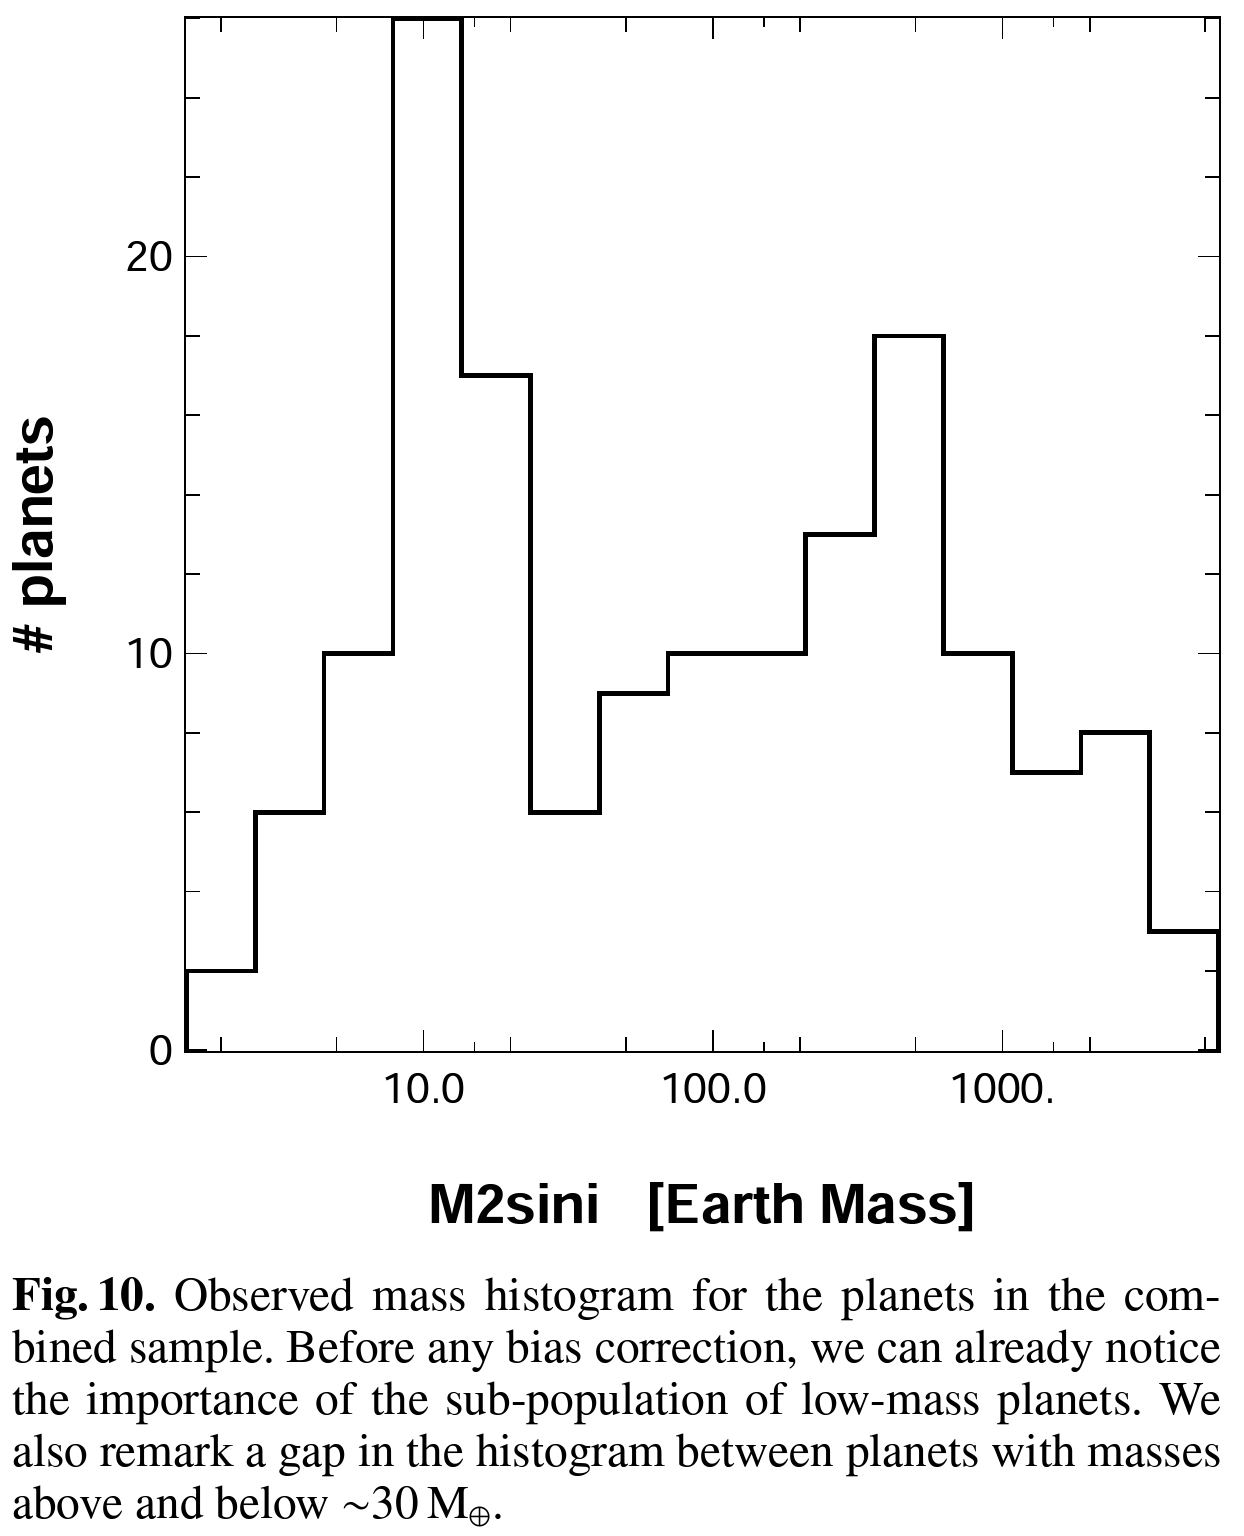
\includegraphics[trim={0cm 0 0 0},clip, height=0.45\textheight]{pvsM} \label{fig:pvsM} \end{subfigure}
~
\begin{subfigure}[b]{0.47\textwidth} \centering 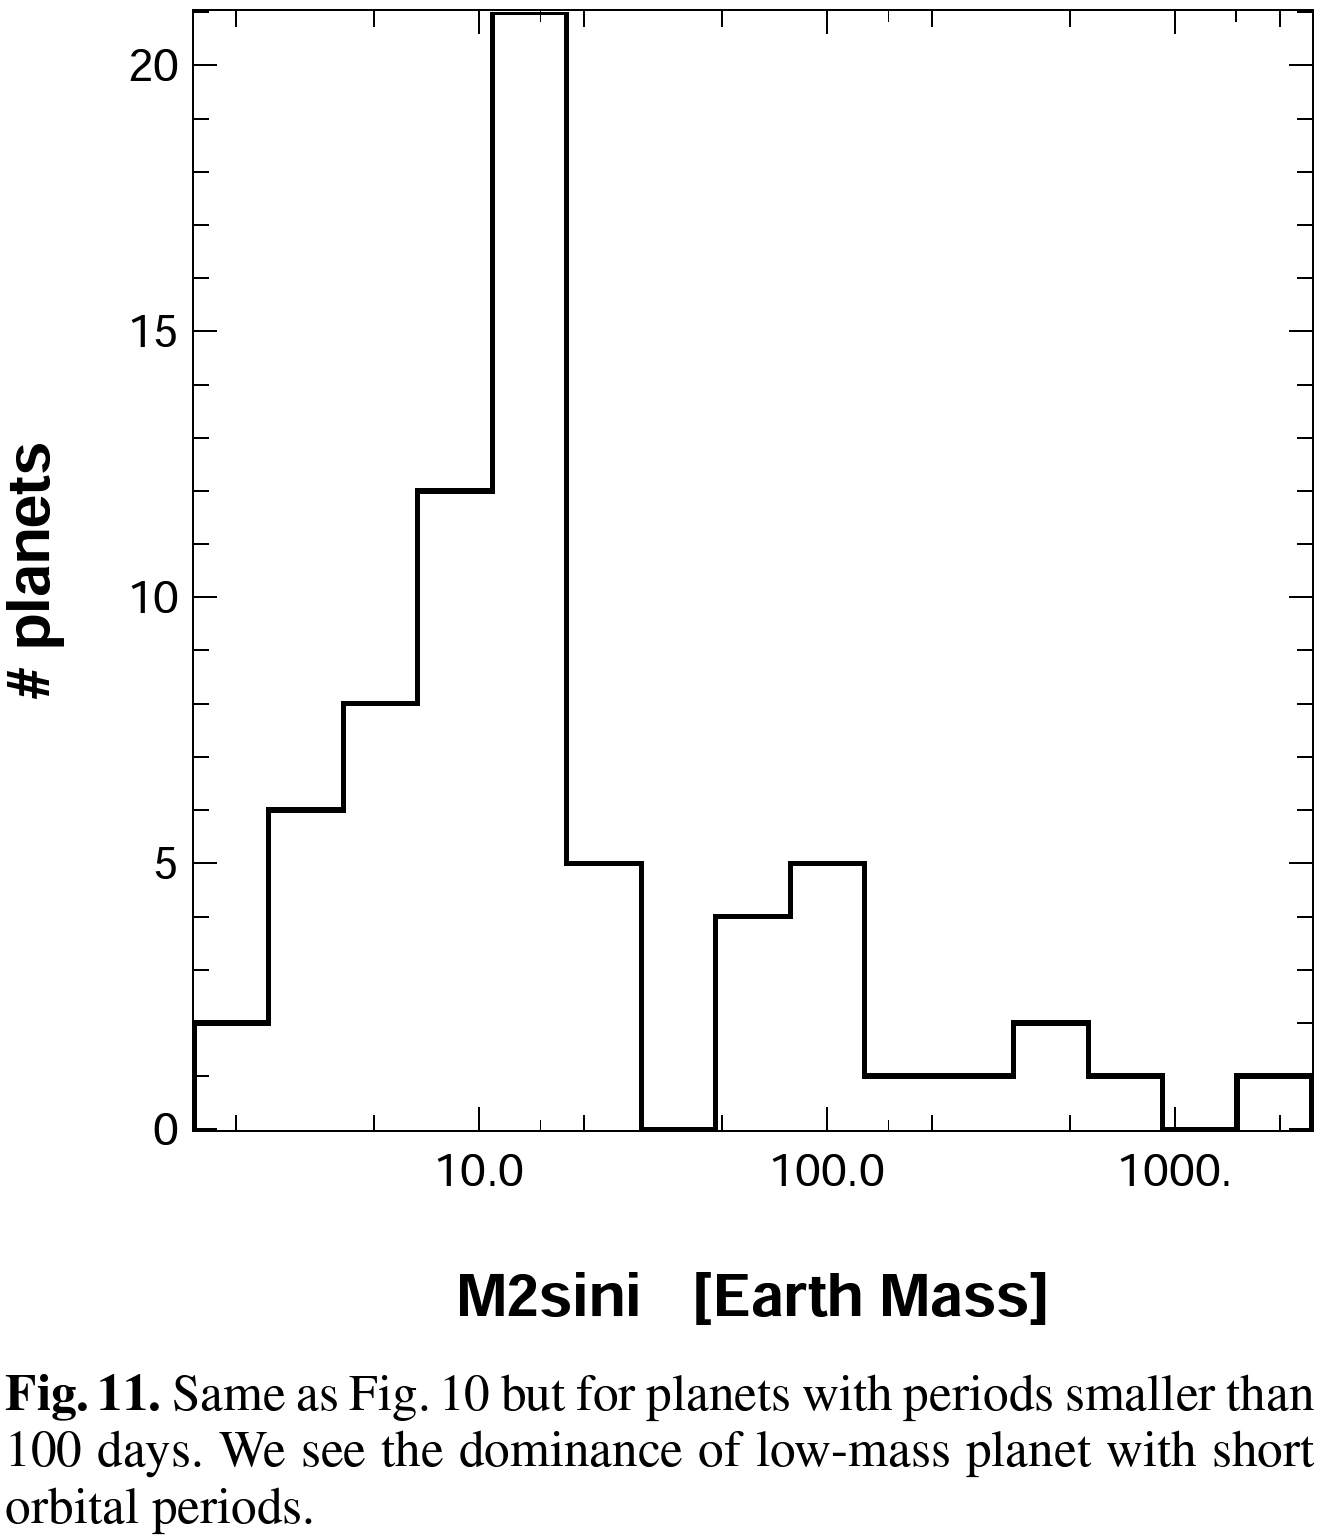
\includegraphics[trim={0cm 0 0 0},clip,height=0.45\textheight]{pvsMP100}\label{fig:pvsMP100}
\end{subfigure}
\end{figure} 

\begin{figure}[!ht]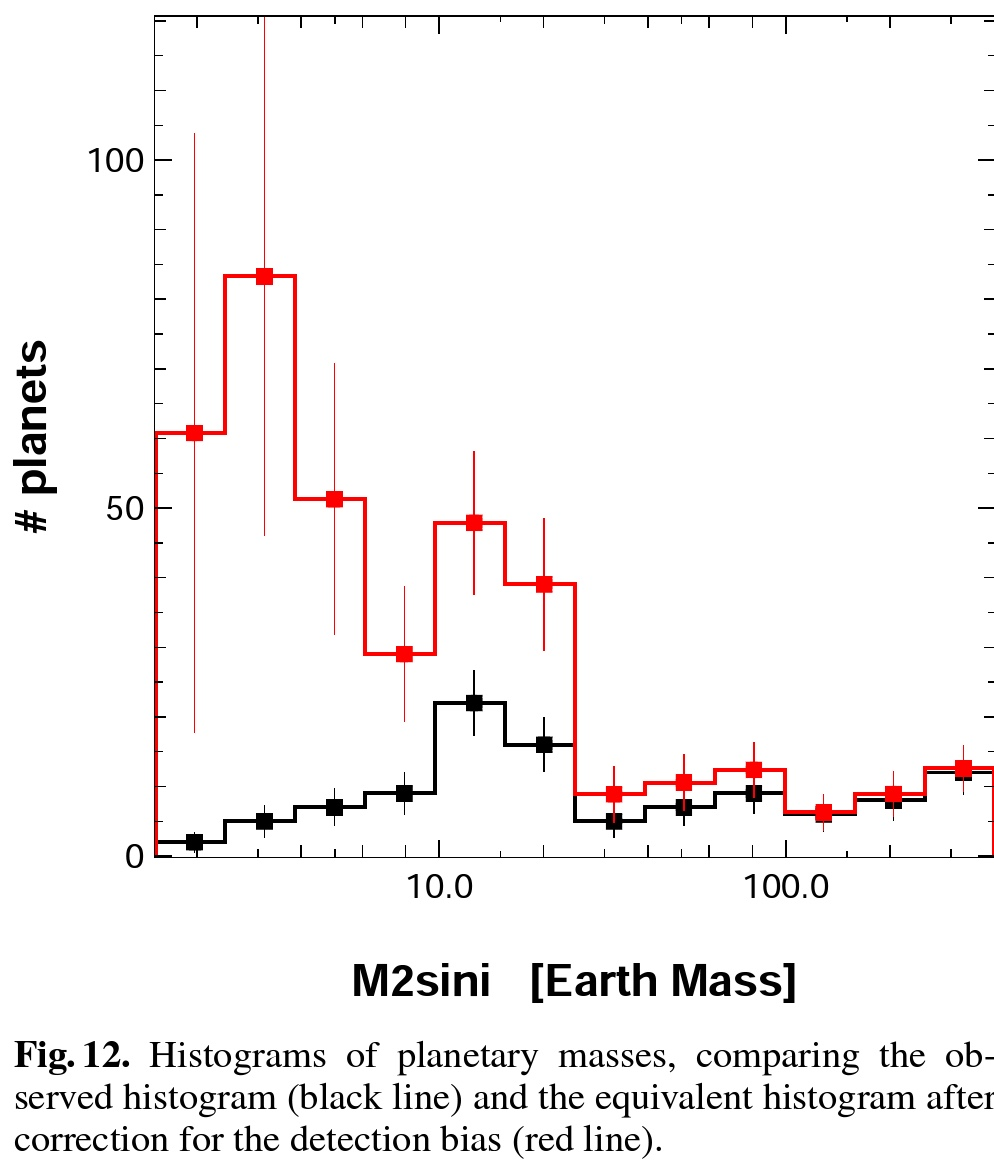
\includegraphics[trim={0cm 0cm 0 0},clip, keepaspectratio,height=0.45\textheight]{freqvsM}\label{fig:freqvsM}
\end{figure}

\end{frame}

\begin{wordonframe}{Distribuzione masse}
Gap nella distribuzione di massa attorno a $30\mearth{}$, popolazione di pianeti con massa minore di $10\mearth{}$ con $P<\SI{100}{\day}$, distribuzione piatta in $\log{M}$ nel range $30\mearth{}-4\mjupiter{}$.
\end{wordonframe}

\begin{frame}{Distribuzione periodi planetarii (a): RV, Mayor 11}
\begin{figure}[!ht]
\begin{subfigure}[b]{0.47\textwidth} \centering 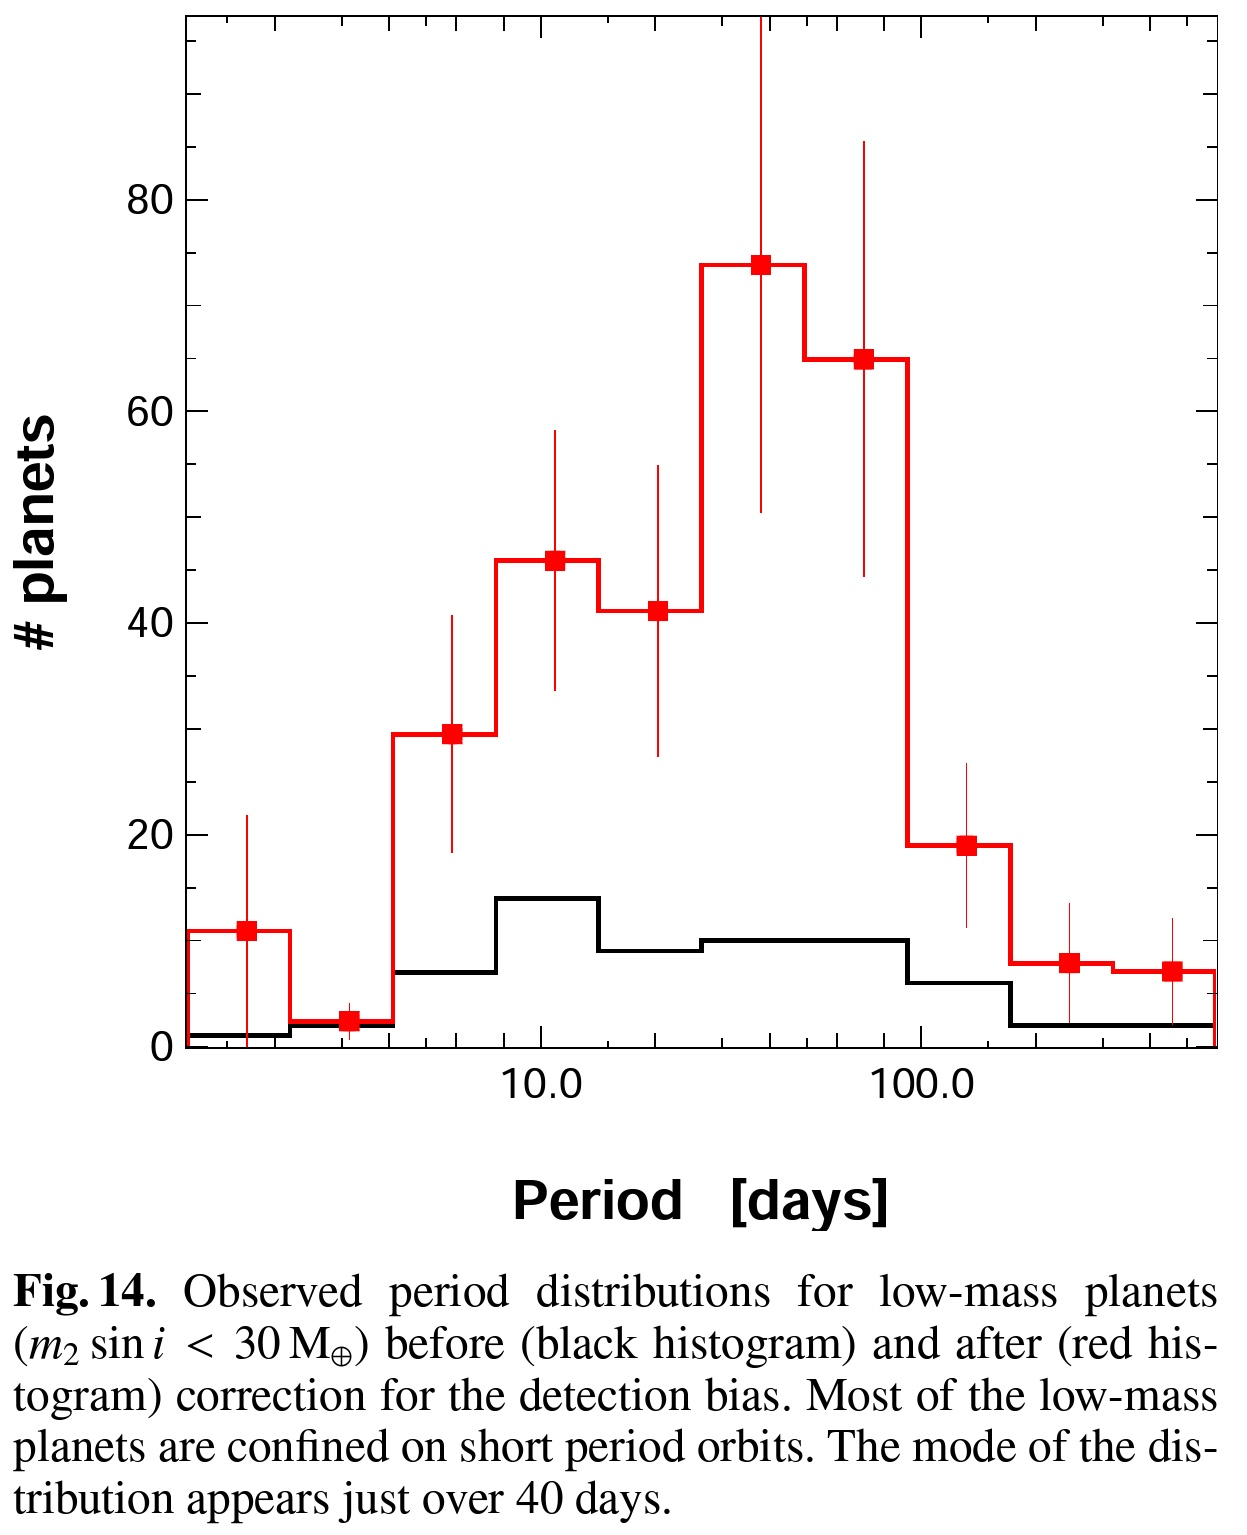
\includegraphics[trim={0cm 0 0 0},clip,width=0.99\textwidth]{freqvsPlowM}\label{fig:freqvsPlowM}\end{subfigure}
~
\begin{subfigure}[b]{0.47\textwidth} \centering 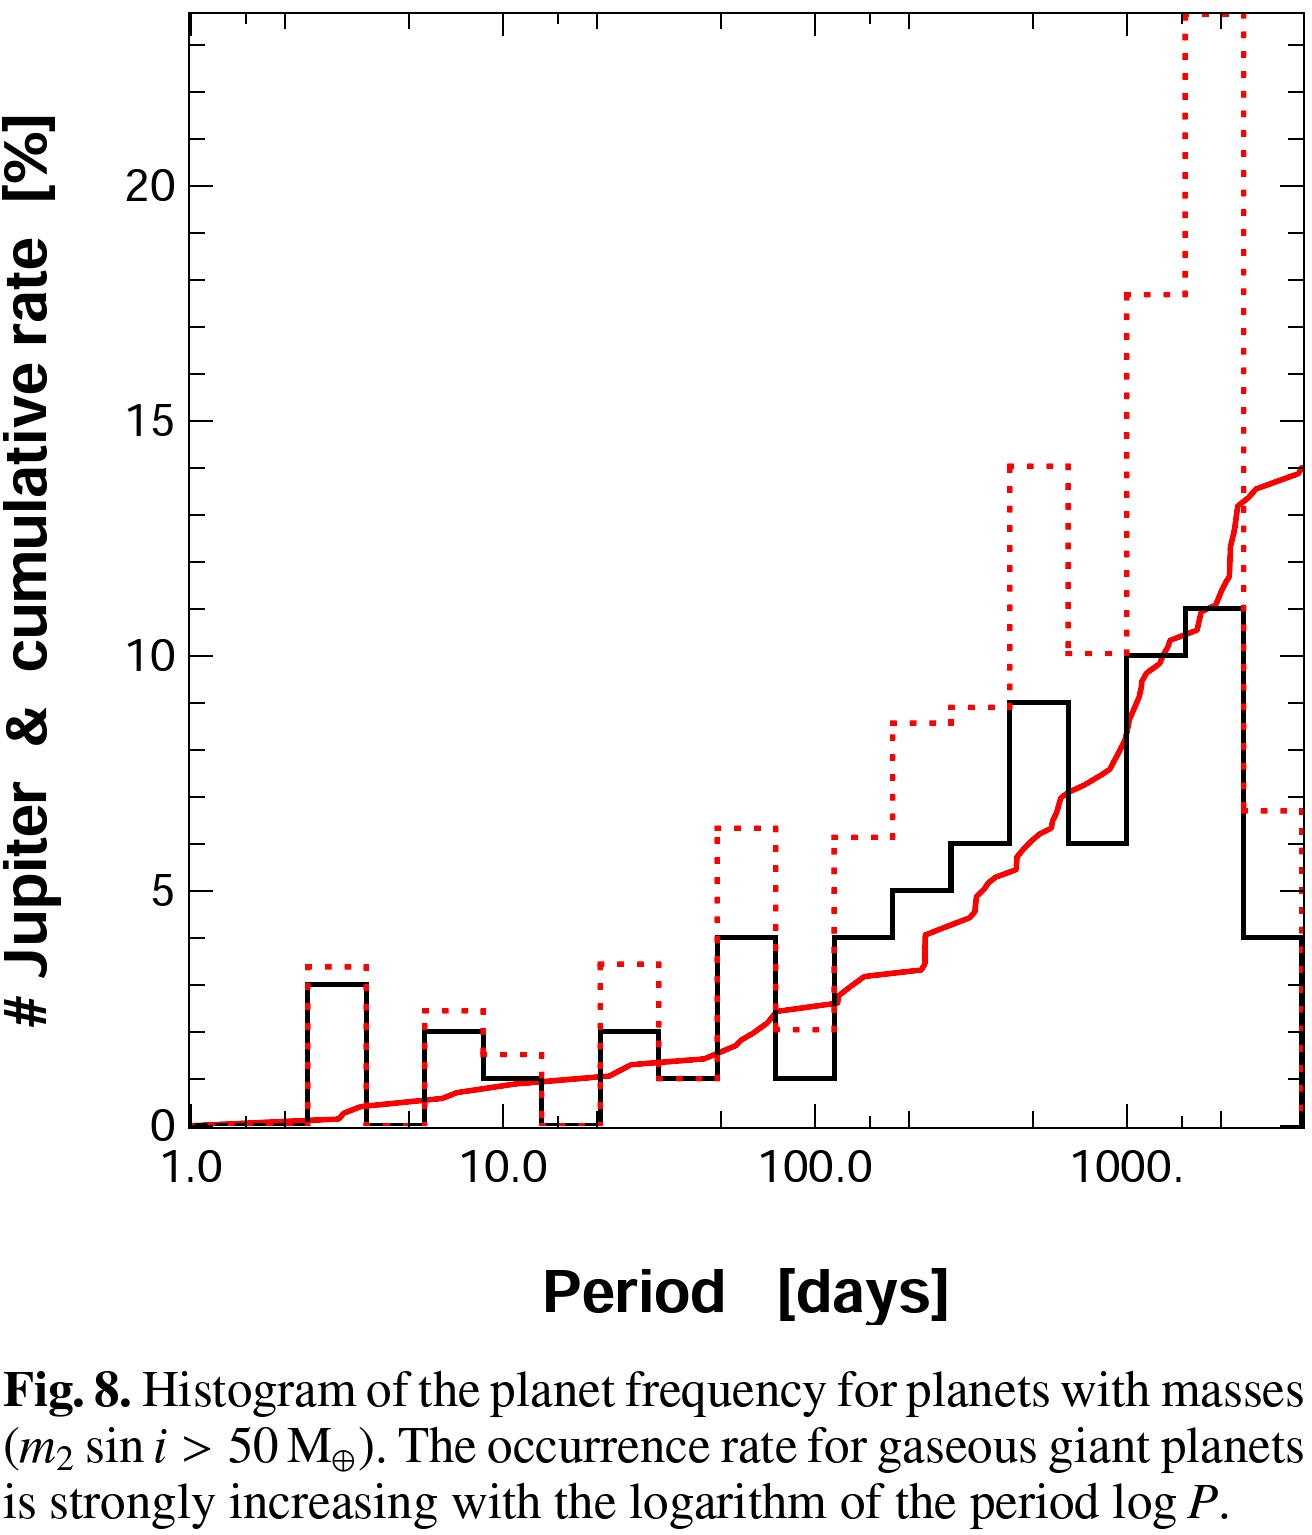
\includegraphics[trim={0cm 0 0 0},clip, height=0.5\textheight]{freqvsPgiant} \label{fig:freqvsPgiant} \end{subfigure}
\end{figure}
\end{frame}

\begin{wordonframe}{Distribuzione periodi}
I pianeti giganti sono raggruppati attorno a \SI{3}{\day}, possibile minimo entro \SI{100}{\day} e distribuzione che cresce rapidamente dopo \SI{100}{\day}.
Pianeti $M<30\mearth{}$ concentrati in \SIrange{10}{100}{\day}.
\end{wordonframe}

\begin{frame}{Caratteristiche orbitali: RV, Mayor 11}
\begin{figure}[!ht]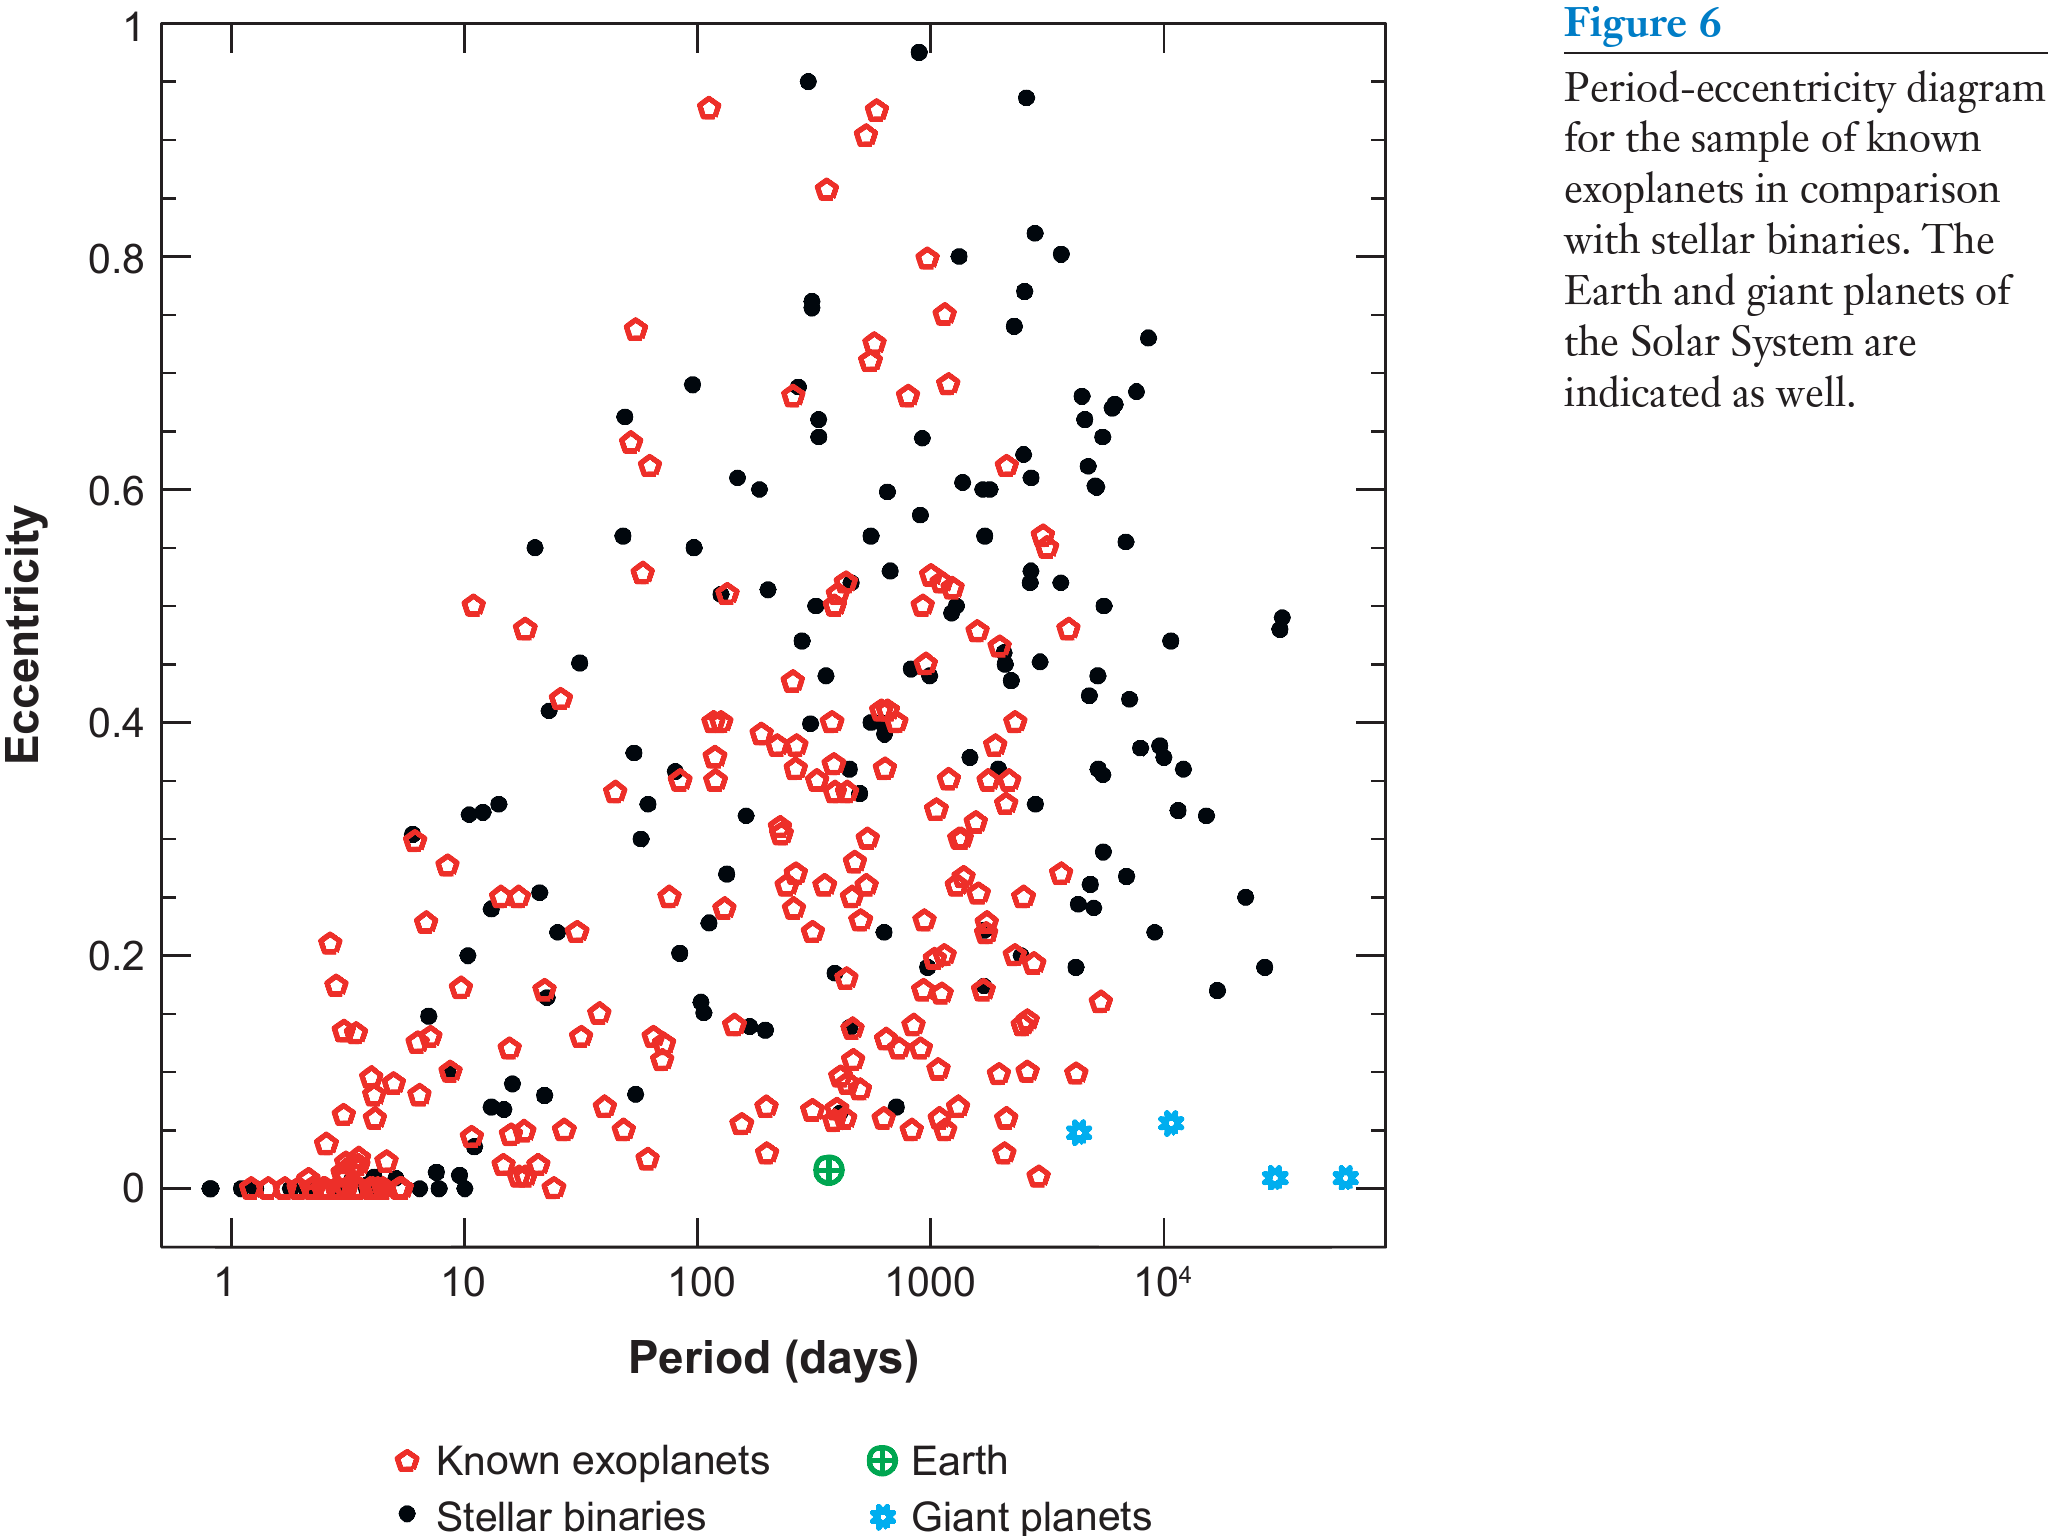
\includegraphics[trim={0cm 0cm 0 0},clip, keepaspectratio,width=0.5\textwidth]{eP}\label{fig:eP}\end{figure}
$\exv{e}\approx0.29$ - binary stars.

\begin{columns}[T]\begin{column}{0.5\textwidth}
Large scattering of e for gas giant (up to 0.93), up to $0.45$ for $M<30\mearth{}$.
\end{column} \begin{column}{0.5\textwidth}
\begin{equation*}
dN=S(x,\sigma_x)\,dx=\frac{x}{\sigma_x^2}\exp{-\frac{x^2}{2\sigma_x^2}} 
\end{equation*}
\end{column}  \end{columns}

\end{frame}

\begin{wordonframe}{Propriet\'a orbitali}
Fuori dalla regione di circolarizzazione mareali, $P=\SIrange{10}{30}{\day}$, ci sono comunque sistemi con piccola e (Sistema solare): evoluzione nel disco proto-planetario.
Sistemi con grande eccentricit\'a con $P=\SIrange{6}{10}{\day}$: influenza di compagno a grande periodo.
Planet-Planet scattering: upper part follow Rayleigh distribution.
\end{wordonframe}

\begin{frame}{Sistemi multipli e metallicit\'a}

\begin{figure}[!ht]
\begin{subfigure}[b]{0.47\textwidth} \centering 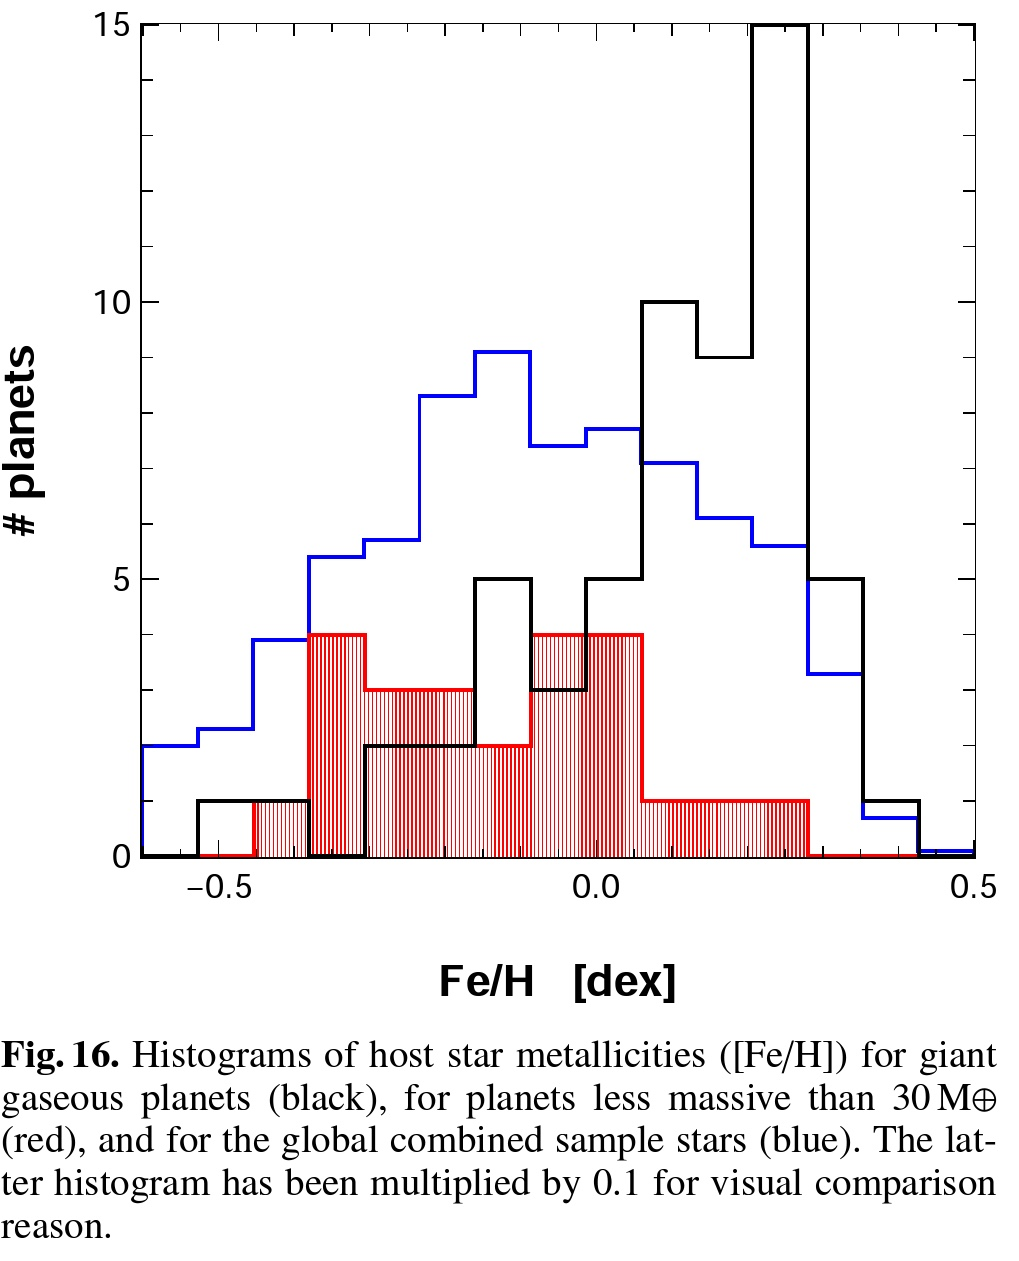
\includegraphics[trim={0cm 0 0 0},clip, height=0.45\textheight]{pvsFeH}\label{fig:pvsFeH} \end{subfigure}
~
\begin{subfigure}[b]{0.47\textwidth} \centering 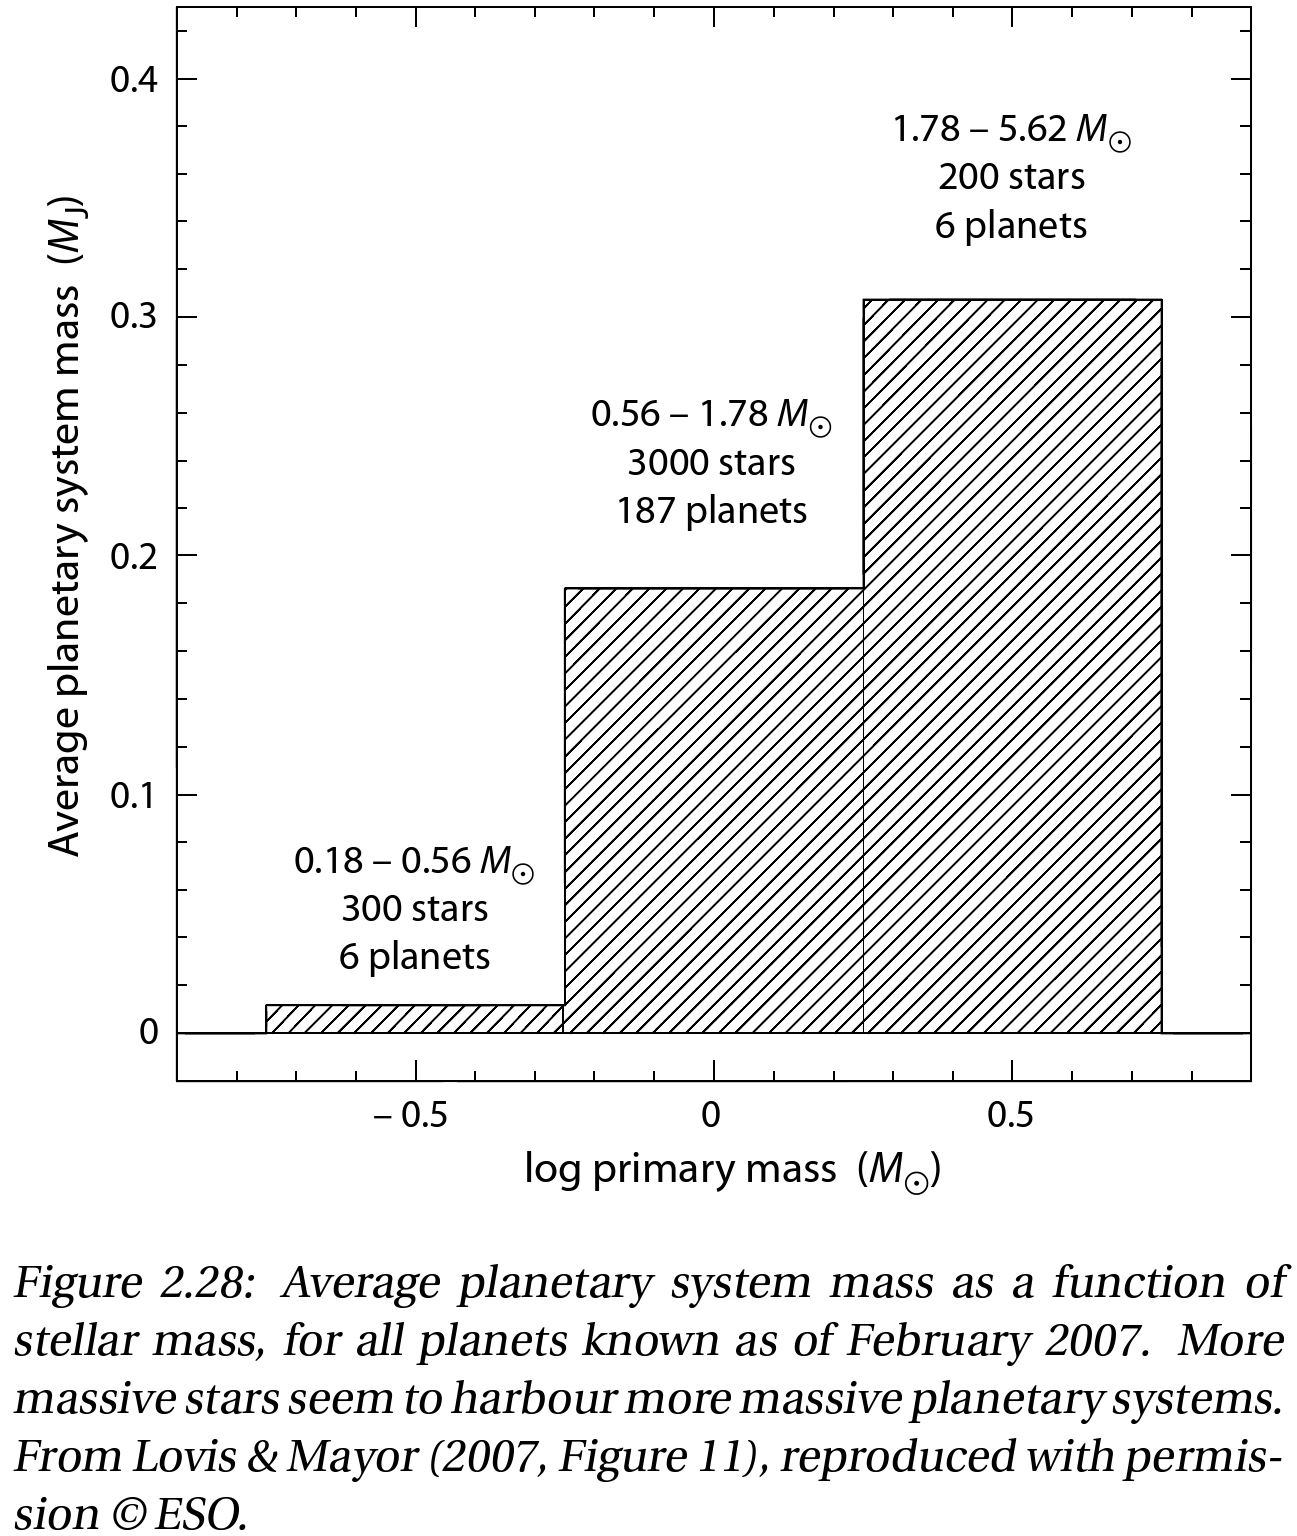
\includegraphics[trim={0cm 0 0 0},clip,height=0.45\textheight]{pMstar}\label{fig:pMstar}\end{subfigure}
\end{figure}
\begin{figure}[!ht]
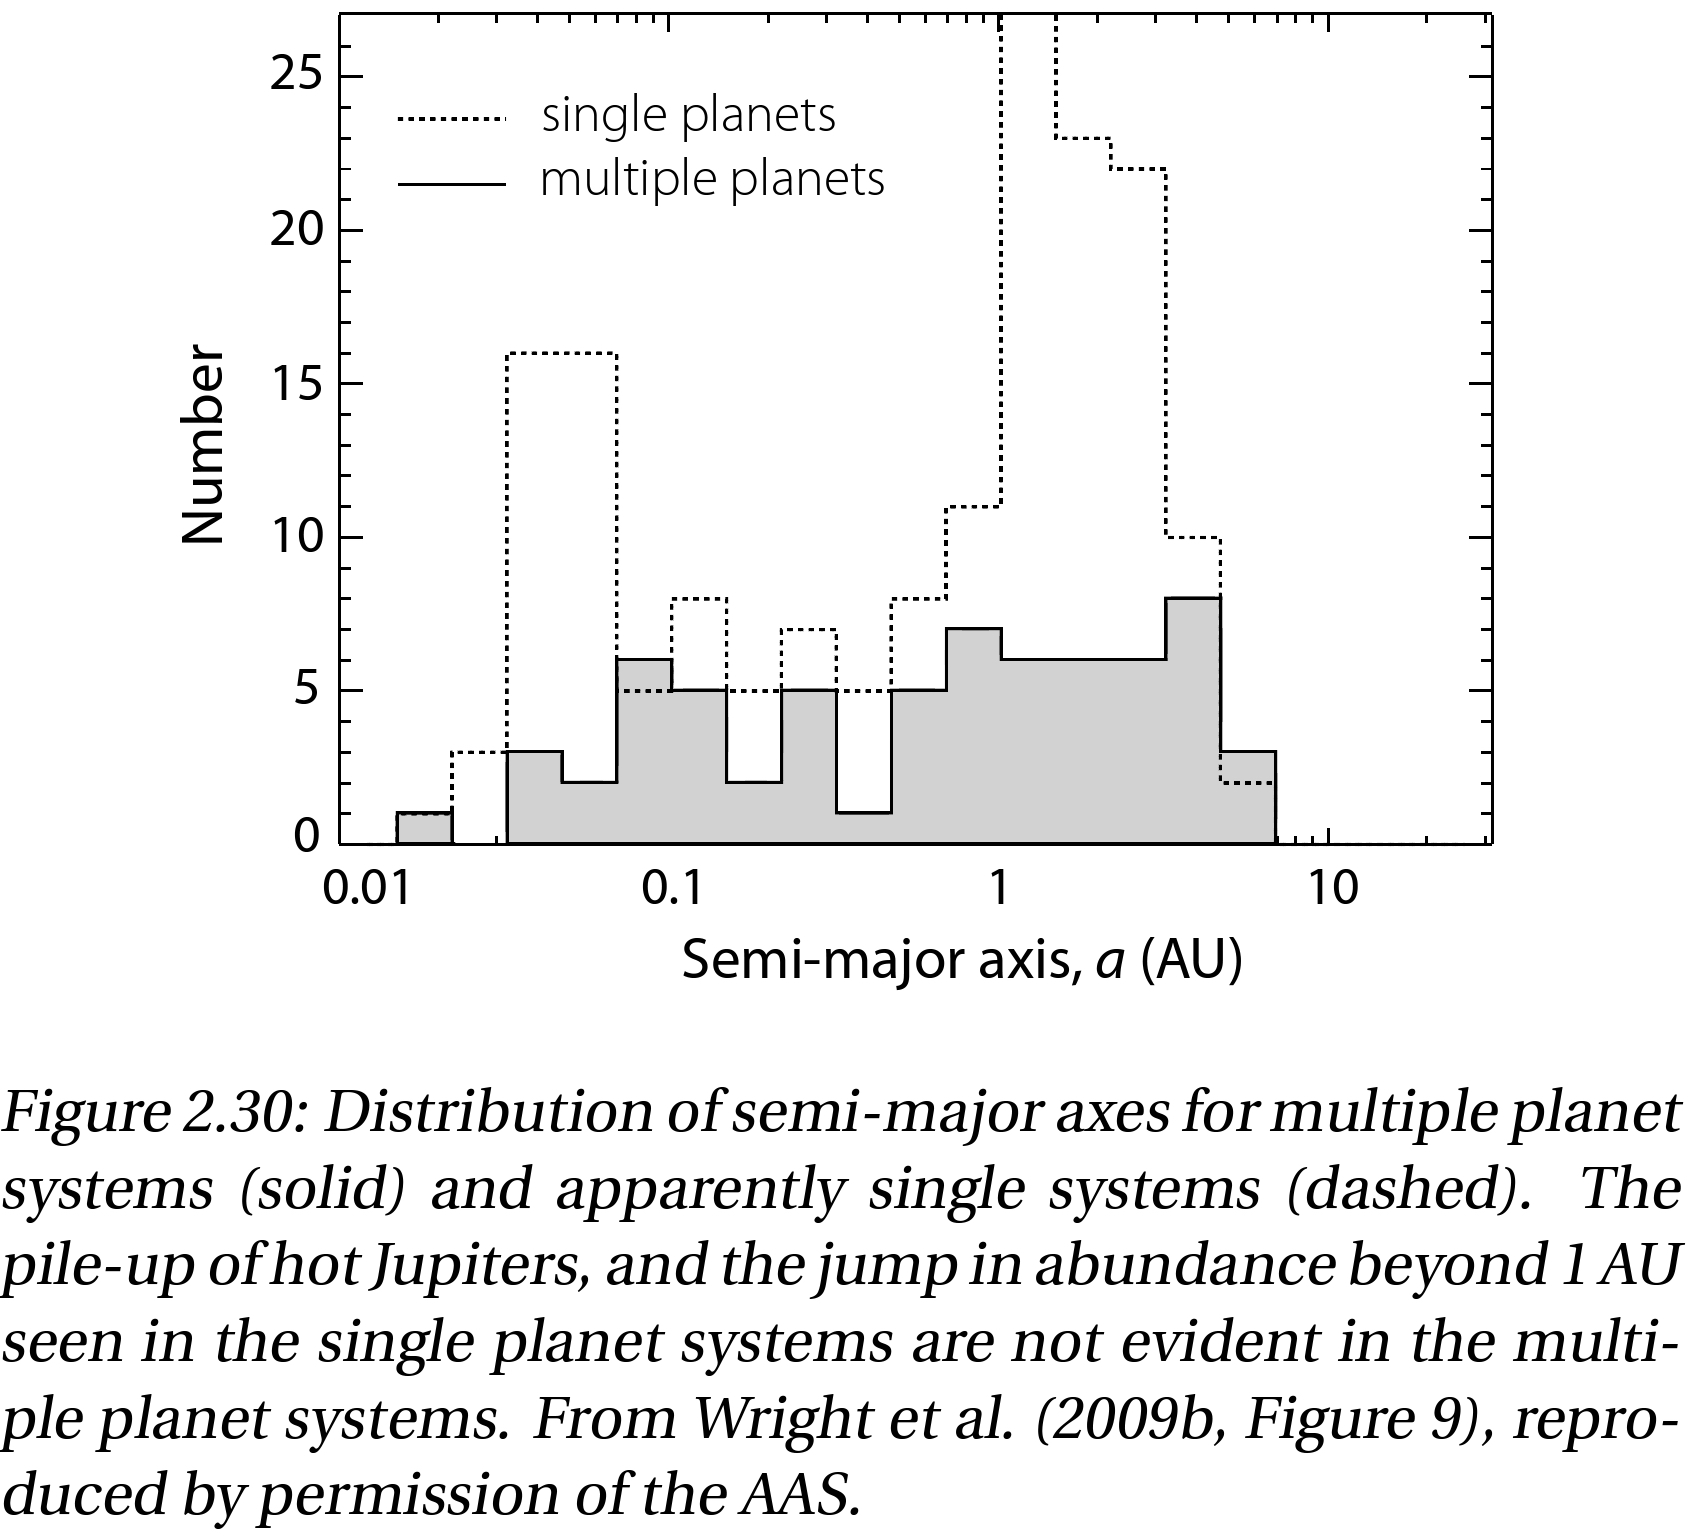
\includegraphics[trim={0cm 0cm 0 0},clip, keepaspectratio,height=0.45\textheight]{a-single-multi}\label{fig:a-single-multi}\end{figure}
\end{frame}

\begin{wordonframe}{Correlazione con caratteristiche stellari e sistemi multipli}
La frequenza dei pianeti giganti aumenta con la metallicit\'a stellare (Santos 04, Fischer Valenti 05); inoltre cresce nel range $1-2\msun{}$.
I sistemi multipli possono essere classificati in maniera non esclusiva secondo il numero di pianeti giganti, la presenza di MMR, secondo l'importanza delle interazioni pianeta-pianeta, la presenza di pianeti sub-gioviani.
La distribuzione dei periodi nei sistemi multipli mostra accumulo meno pronunciato a \SI{3}{\day}, e \SI{1}{\astronomicalunit}
\end{wordonframe}


\section{Properties of transit exoplanets}

\begin{frame}{Distribuzione raggio planetario}
\begin{columns}  \begin{column}{0.5\textwidth}
\begin{figure} \centering 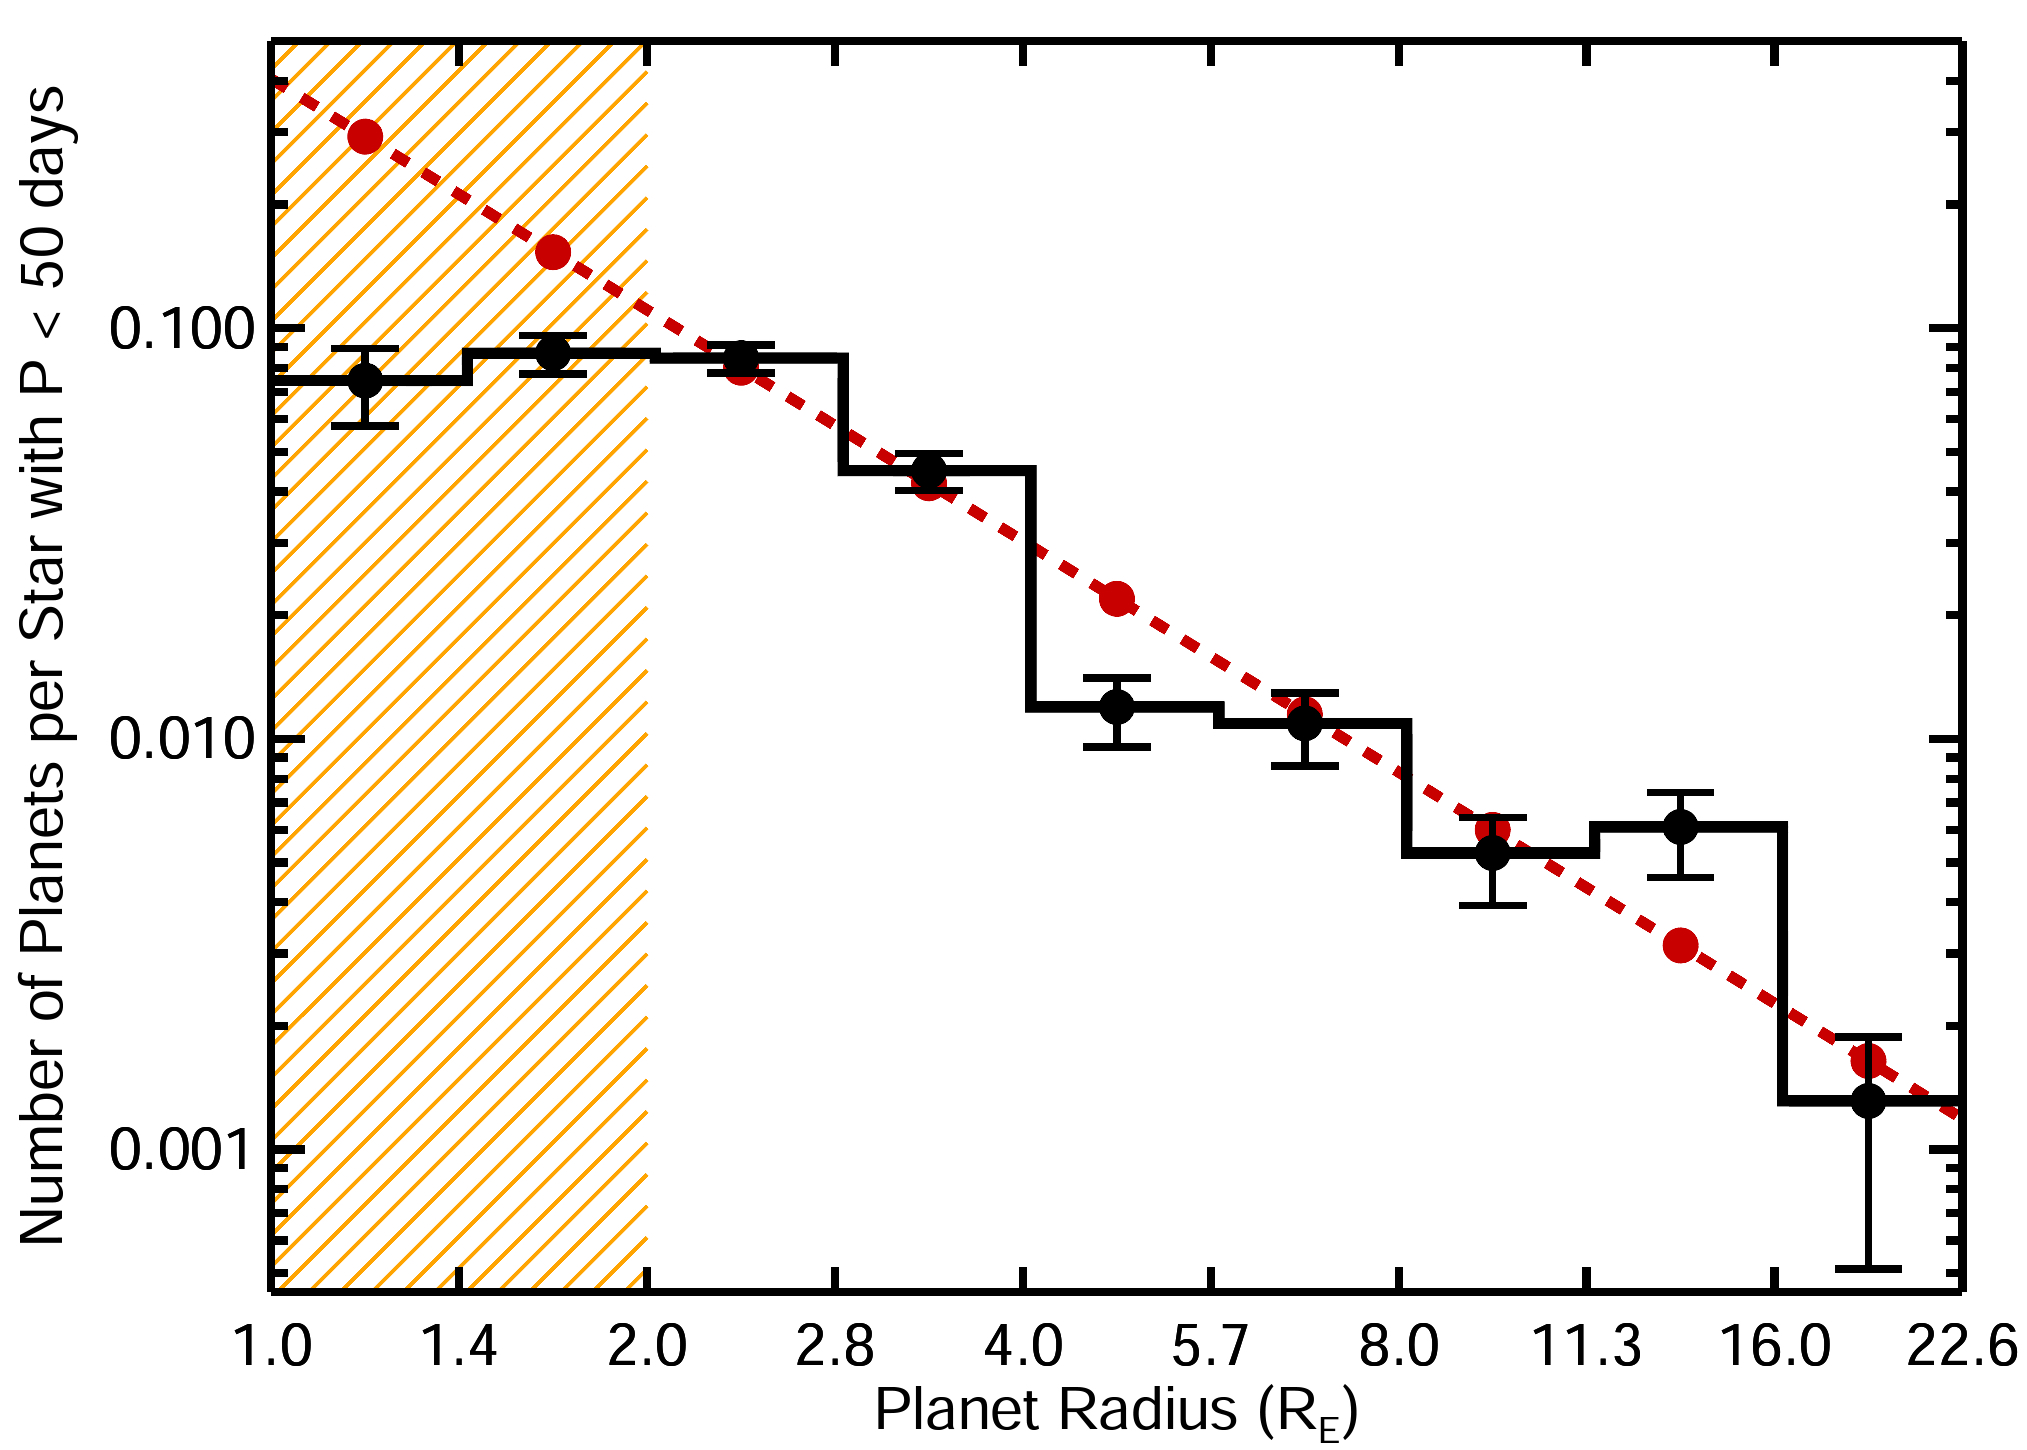
\includegraphics[trim={0cm 0 0 0},clip, height=0.45\textheight]{freqvsRpl50l} \label{fig:freqvsRpl50l}
\end{figure}

\begin{figure}
\centering \includegraphics[trim={0cm 0 0 0},clip,height=0.45\textheight]{freqvsRpl50}\label{fig:freqvsRpl50}\end{figure} 
\end{column} \begin{column}{0.5\textwidth}
\cite{howard2012planet}: $P<\SI{50}{\day}$, $R=\range{2}{22.7}\rearth{}$
\begin{equation*}

\end{equation*}
\end{column}  \end{columns}
\end{frame}

\section{Orbital evolution}

\subsection{Hot Jupiters due to tidal circularization}

\begin{frame}{Planet-Planet scattering}
Scattering in eccentric close-in orbit. Tidal circularization: limit distance twice the Roche limit.
\end{frame}

\begin{wordonframe}{Tidal circularization}
During circularization angular momentum $\propto \sqrt{GMa(1-e^2)}$: for $e\approx1$: $a_f=a_i(1-e^2)\approx2a_{peri}$.

$R_p=0.462a_R(\frac{M_p}{M_*})\expy{\frac{1}{3}}$ 
\end{wordonframe}


\clearpage

%\listofframes

\end{document}